%!TEX root = ../../../adrien_gomar_phd.tex

\subsection{Stability curve}
\label{sub:dream_ls_ael_curve}

The damping as a function the inter-blade phase angle, namely the stability
curve is reported for the two modes considered in Figure~\ref{fig:dream_ls_ael_damping}.
All the modes have a positive damping which clear this low-speed CROR configuration
from flutter. The minimum damping is at IBPA=$30^\circ$ for the second flexion
mode and at IBPA=$-30^\circ$ for the first torsion mode.
The variation of the damping against the inter-blade phase angle is
limited for the 2F mode while a much interval of variation is
observed for the 1T mode. To further analyze the aeroelastic behavior
of the front rotor blades, the local damping is computed.
\begin{figure}[htp]
  \centering
  \subfigure[mode 2F]{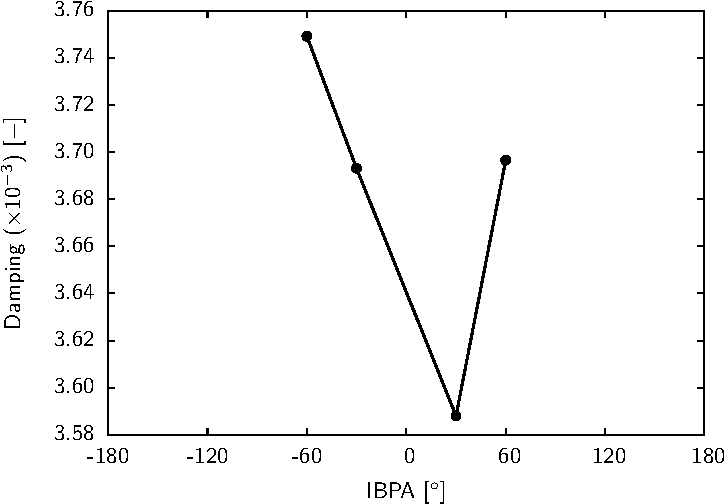
\includegraphics[width=.4\textwidth]{DREAM_LS_DAMPING_MODE_2F.pdf}}
  \subfigure[mode 1T]{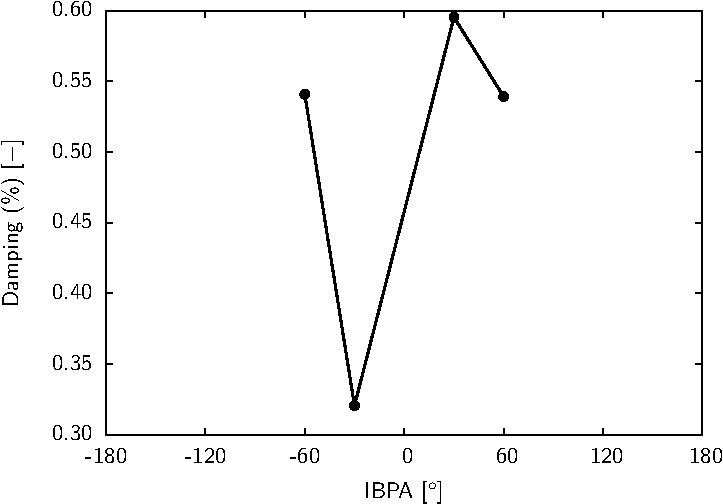
\includegraphics[width=.4\textwidth]{DREAM_LS_DAMPING_MODE_1T.pdf}}
  \caption{Low-speed isolated configuration: integrated damping for modes 2F and 1T.}
  \label{fig:dream_ls_ael_damping}
\end{figure}

\subsection{Local excitation}
\label{sub:dream_ls_ael_local_damping}

The local excitation is shown on the pressure side and
the suction side of the front rotor blades in 
Figure~\ref{fig:dream_ls_ael_local_damping}. It is the
local damping given in each cell divided by the 
surface of the cell. It is therefore expressed in
m\textsuperscript{-2}.

Firstly, the amplitude of variation of the excitation
is confirmed by the local results. In fact, higher excitation peaks
are observed on the 1T mode results. This can be explained
by the physical behavior of the 1T mode. The shape of this last
has the tendency to change the angle of attack of the blade,
which governs at first order the
performance of the blade. Therefore, changing the angle of attack
of the blades can have a strong impact on the flow field
that develops around the blades. This can explain why the
first torsion mode damping has a larger variation interval
compared to the second flexion mode.

Secondly, the variation of the excitation against IBPA
is barely seen for the 2F mode. The shape of the
results does not change. This is not true for the
1T mode. At the leading edge of the pressure side,
a positive excitation structure is seen for all inter-blade phase
angles except
\mbox{IBPA$=-30^\circ$}. Moreover, for this last, 
the two biggest excitation structures on the pressure 
and suction sides seem to propagate toward the hub.

Thirdly, inflexion lines
for the modes are also inflexion lines for the local excitation
value. Moreover, inflexion lines for the flow physics as the
strong adverse pressure gradient near the leading edge of the blade
on the pressure side that lessened at approximately $25\%$ of the chord
is a region were the local excitation changes in terms of sign.
This effect is not seen on the pressure side where the flow physics
is smoother than on the suction side of the blades. Even though the
local excitations values on the 1T mode are higher in terms of
intensity, this is not observed in the damping value that
has the same order of magnitude than the one of the 2F mode.
Only the variation of damping between different inter-blade phase angles
is affected. 

\begin{figure}[htp]
 \ra{1.3} \centering
 \begin{tabular}{r|cccc}
   \toprule
   & \multicolumn{4}{c}{
        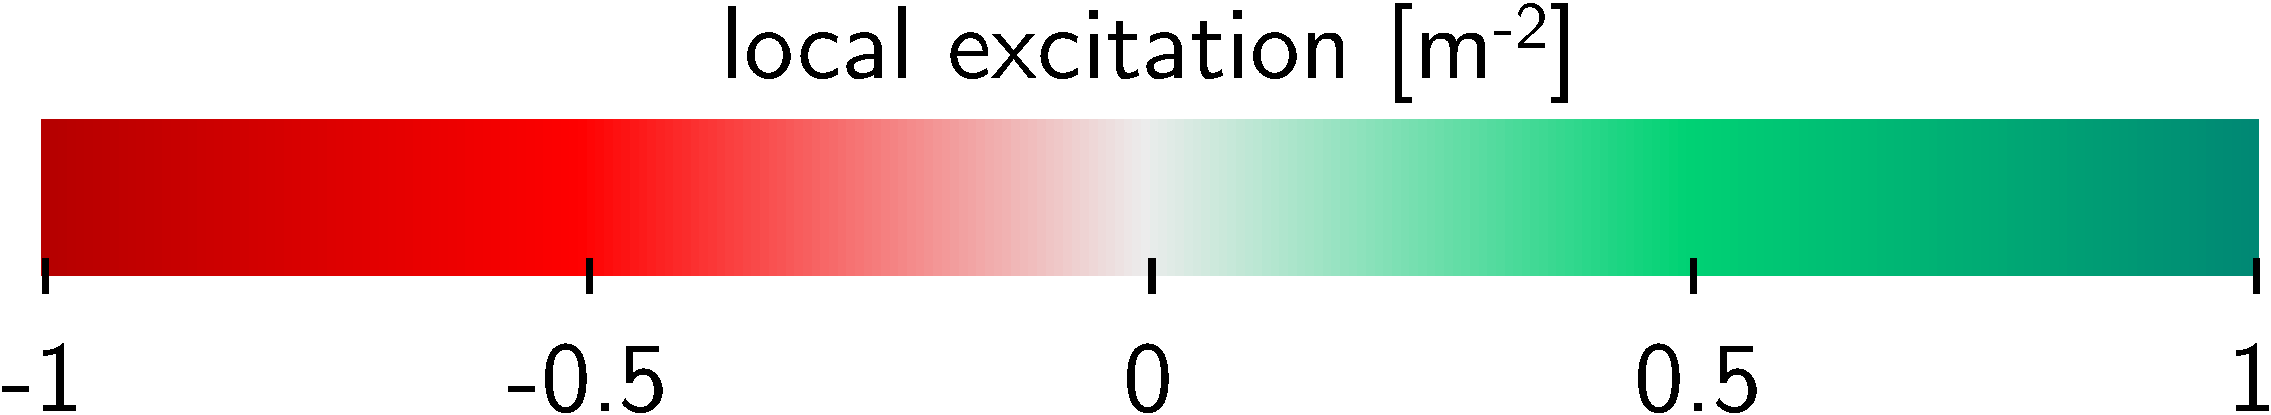
\includegraphics[width=0.22\textwidth]{dream_ls_damping_scale.pdf}} \\
   & \multicolumn{2}{c}{mode 2F} & \multicolumn{2}{c}{mode 1T} \\
   \midrule
   \rotatebox{90}{\quad\quad\quad IBPA $= -60^\circ$} 
   & 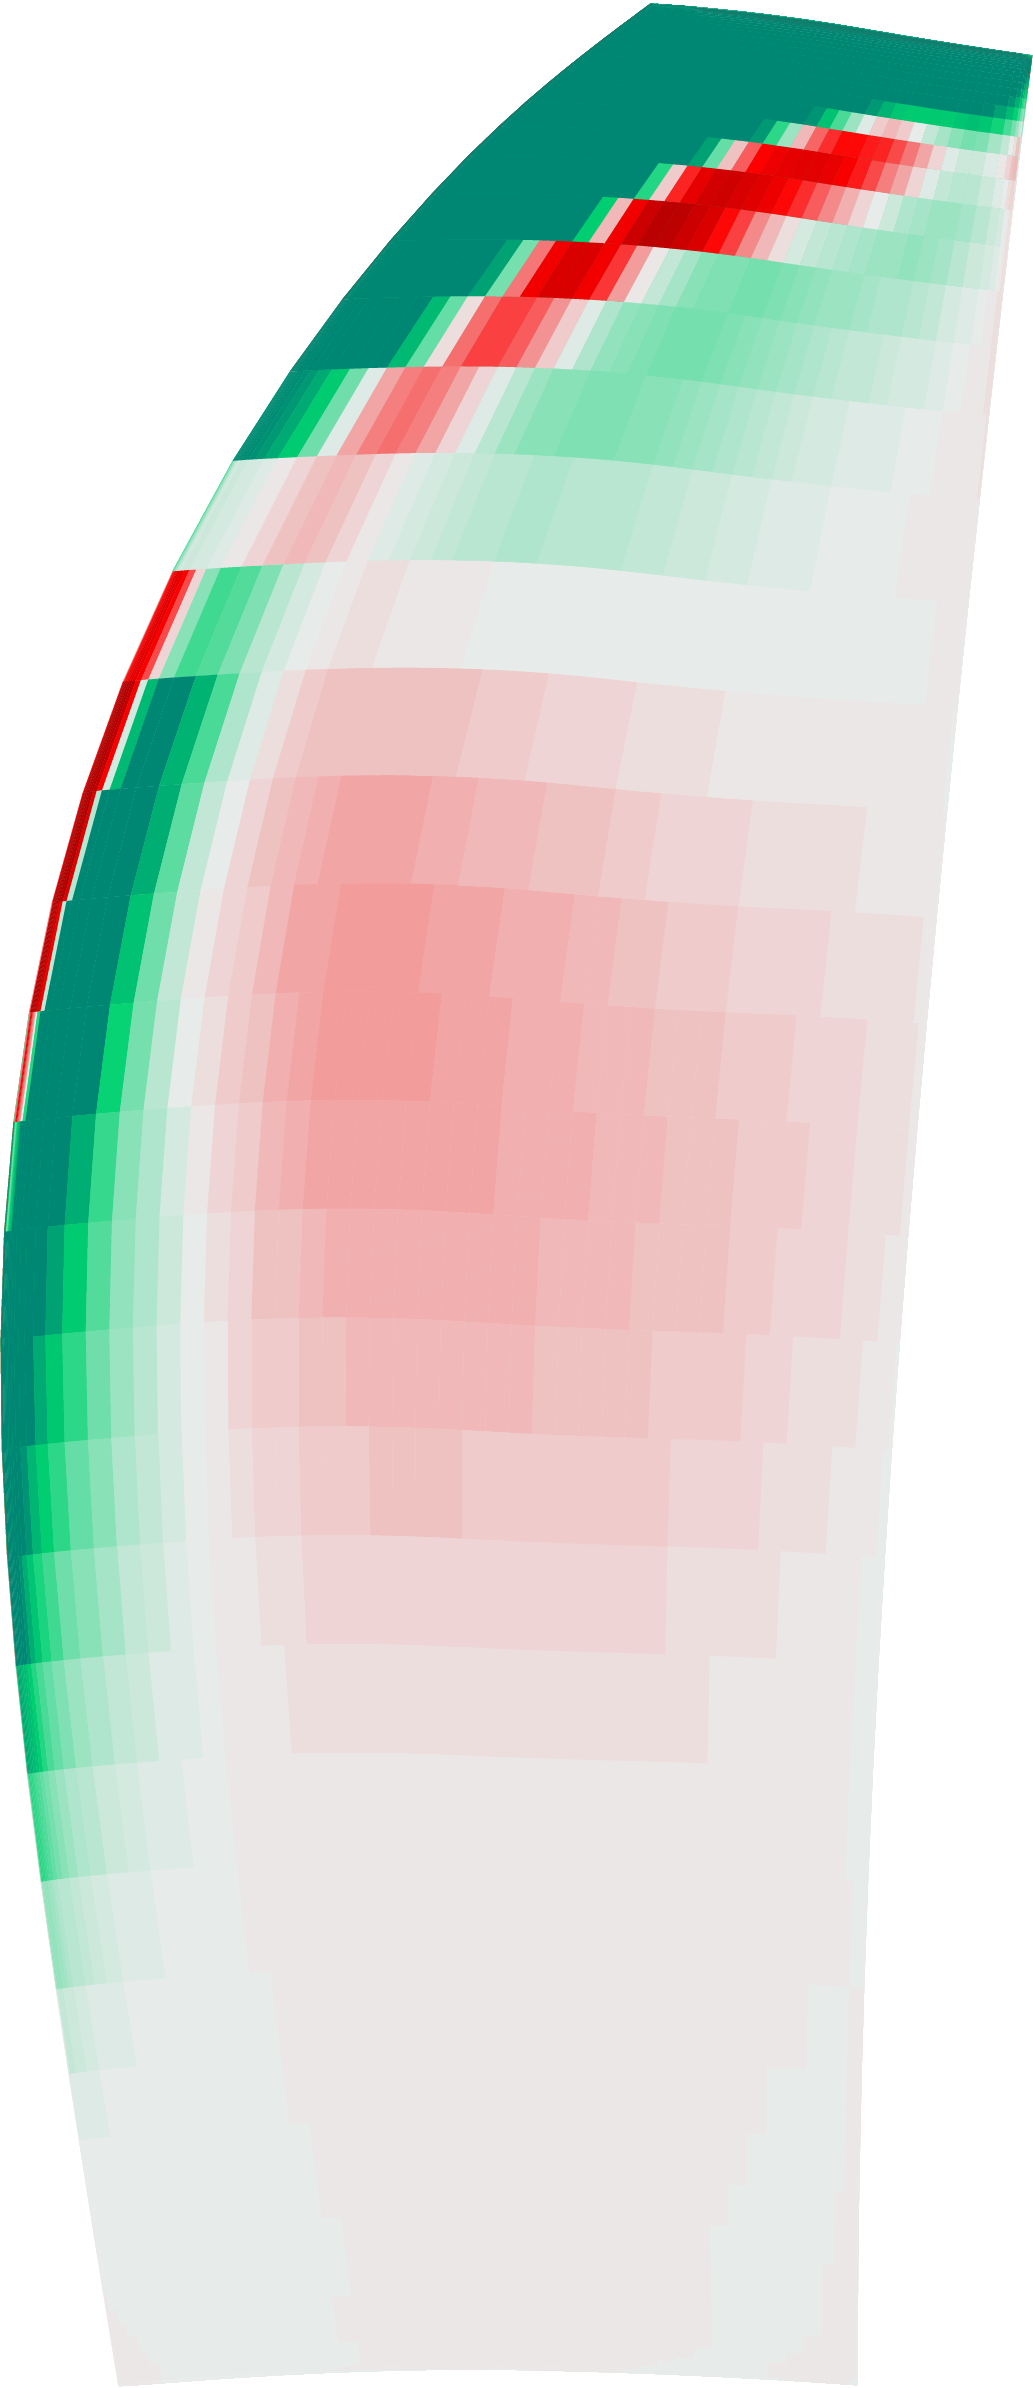
\includegraphics[width=0.12\textwidth]{DREAM_LS_HBT_N5_AEL_H1M2FD-3_roe3_sa_local_damping_SS.png}
   & 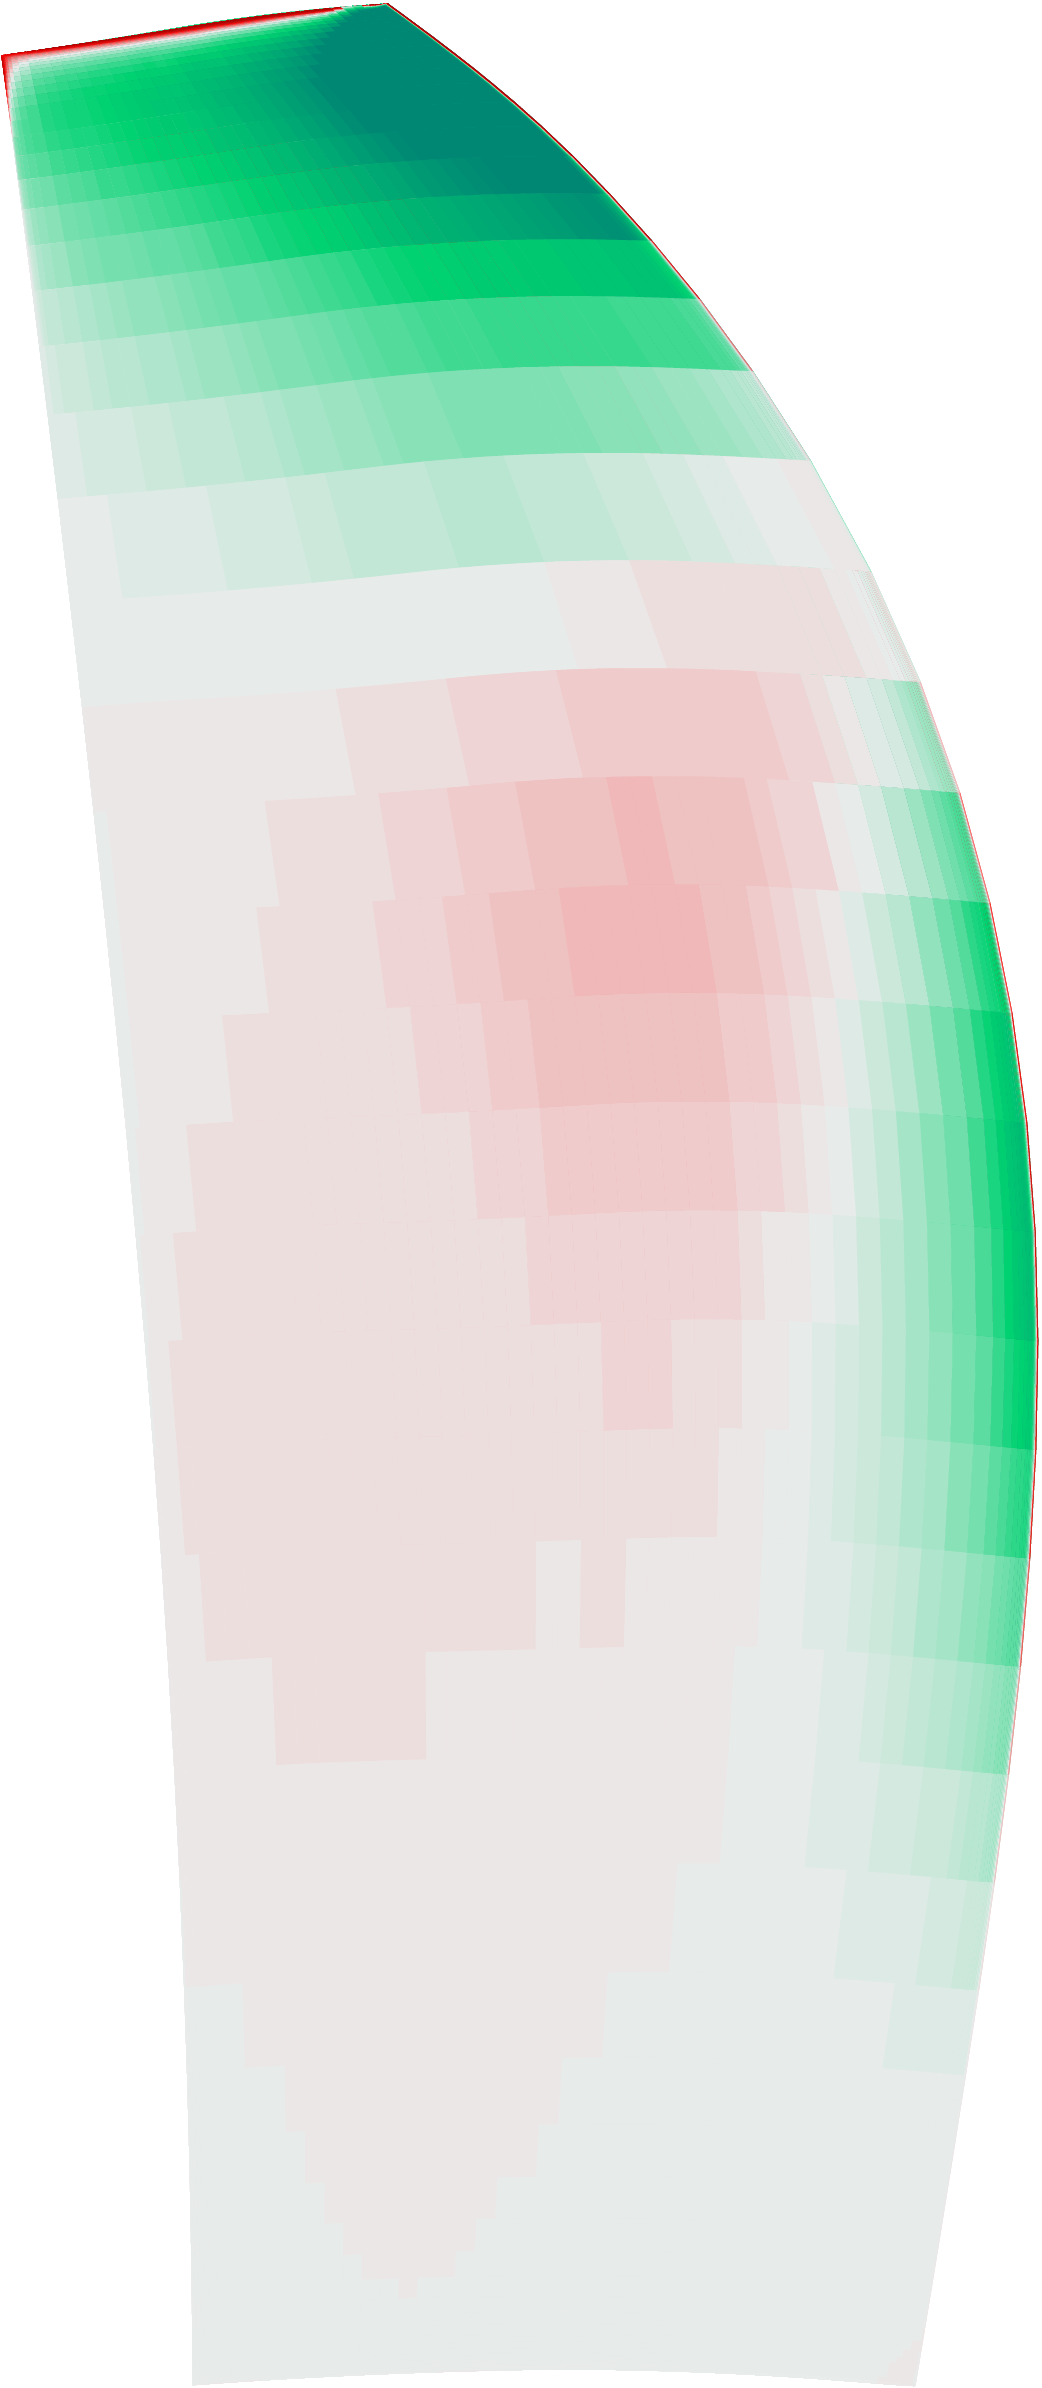
\includegraphics[width=0.12\textwidth]{DREAM_LS_HBT_N5_AEL_H1M2FD-3_roe3_sa_local_damping_PS.png}
   & 
\includegraphics[width=0.12\textwidth]{DREAM_LS_HBT_N5_AEL_H1M1TD-3_roe3_sa_local_damping_SS.png}
   & 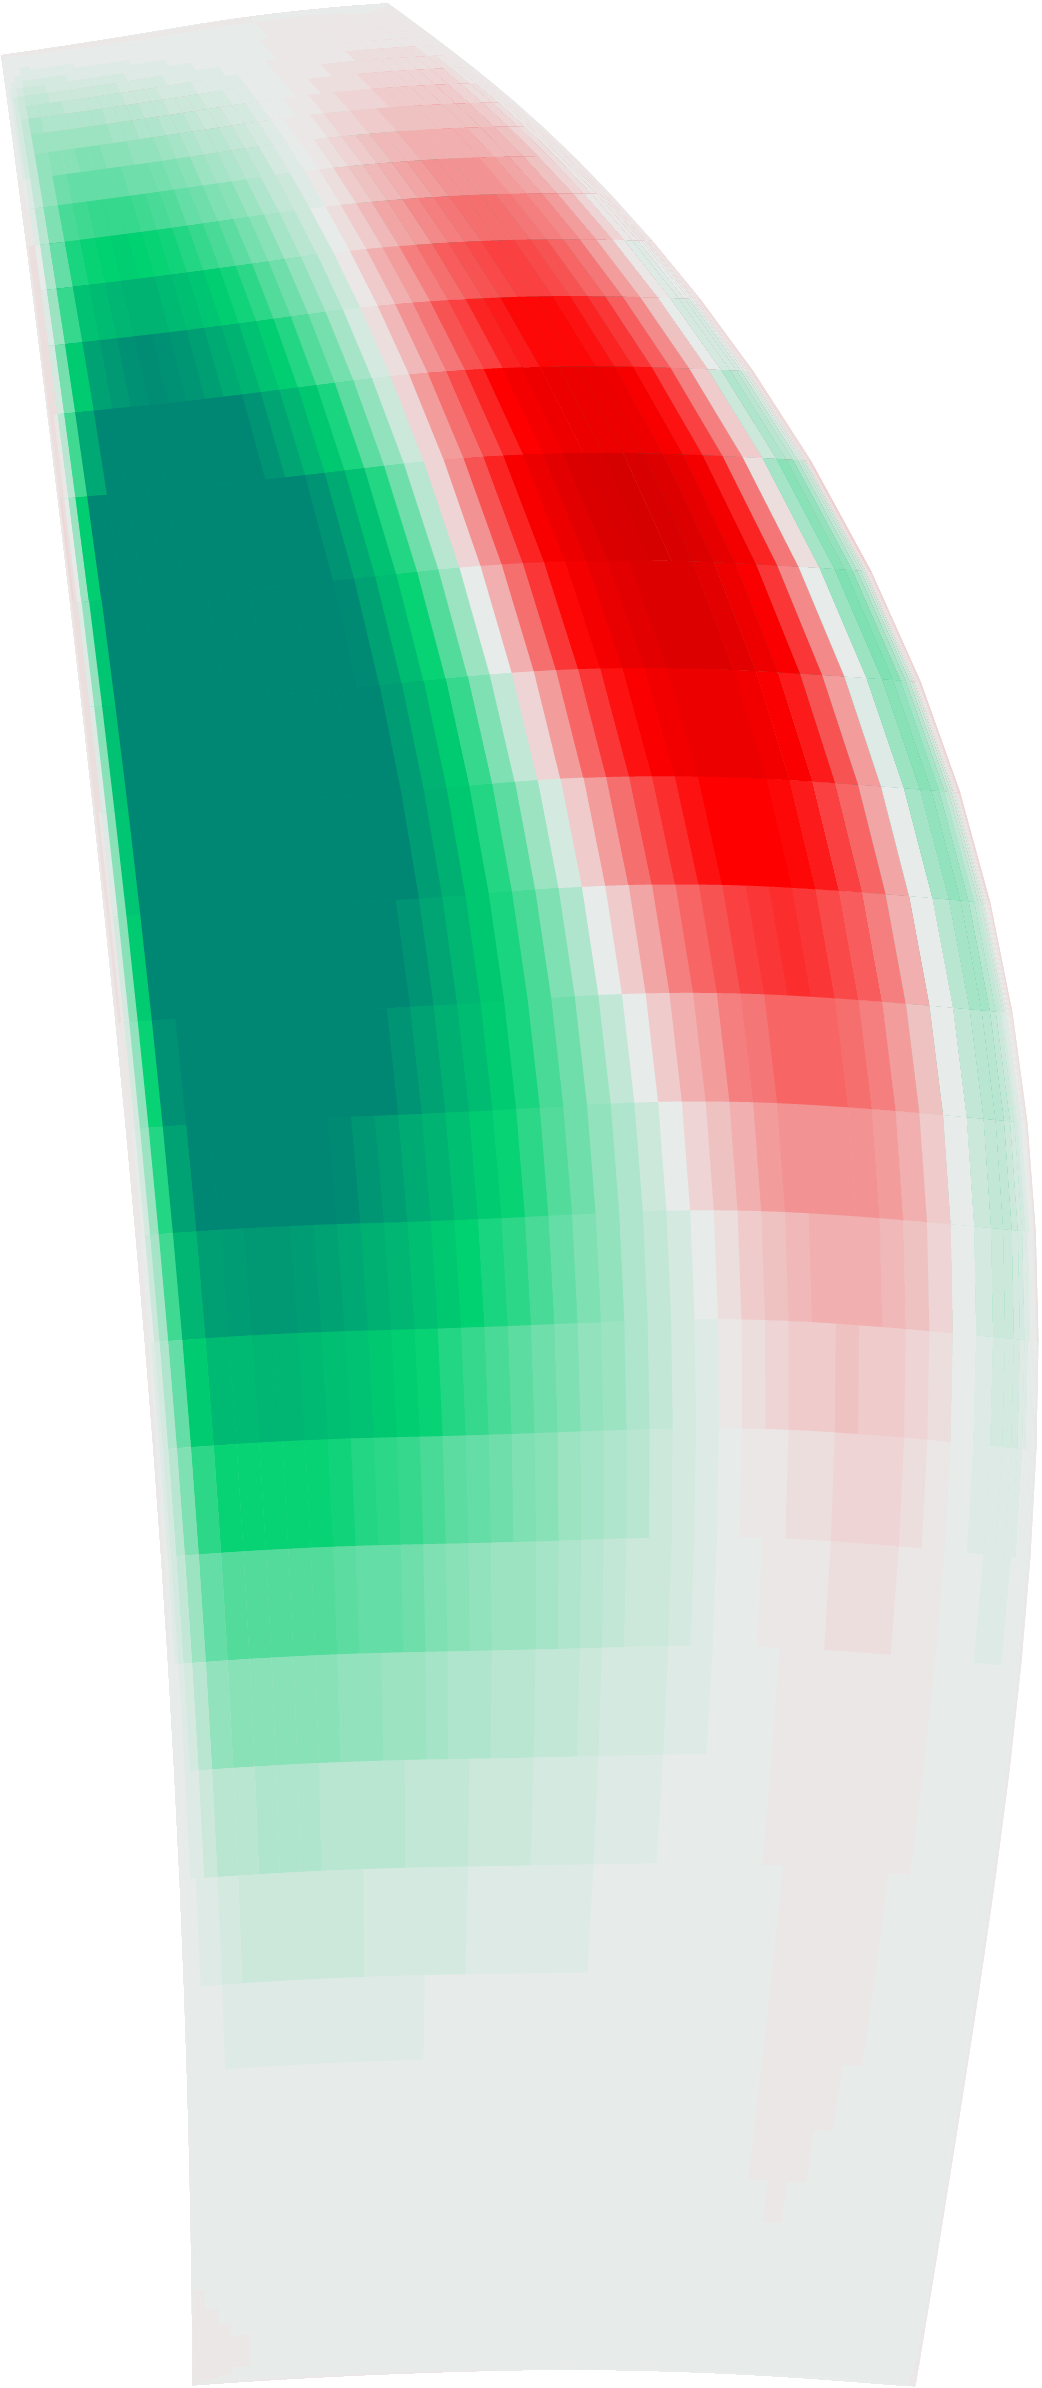
\includegraphics[width=0.12\textwidth]{DREAM_LS_HBT_N5_AEL_H1M1TD-3_roe3_sa_local_damping_PS.png} \\
   \rotatebox{90}{\quad\quad\quad IBPA $= -30^\circ$} 
   & 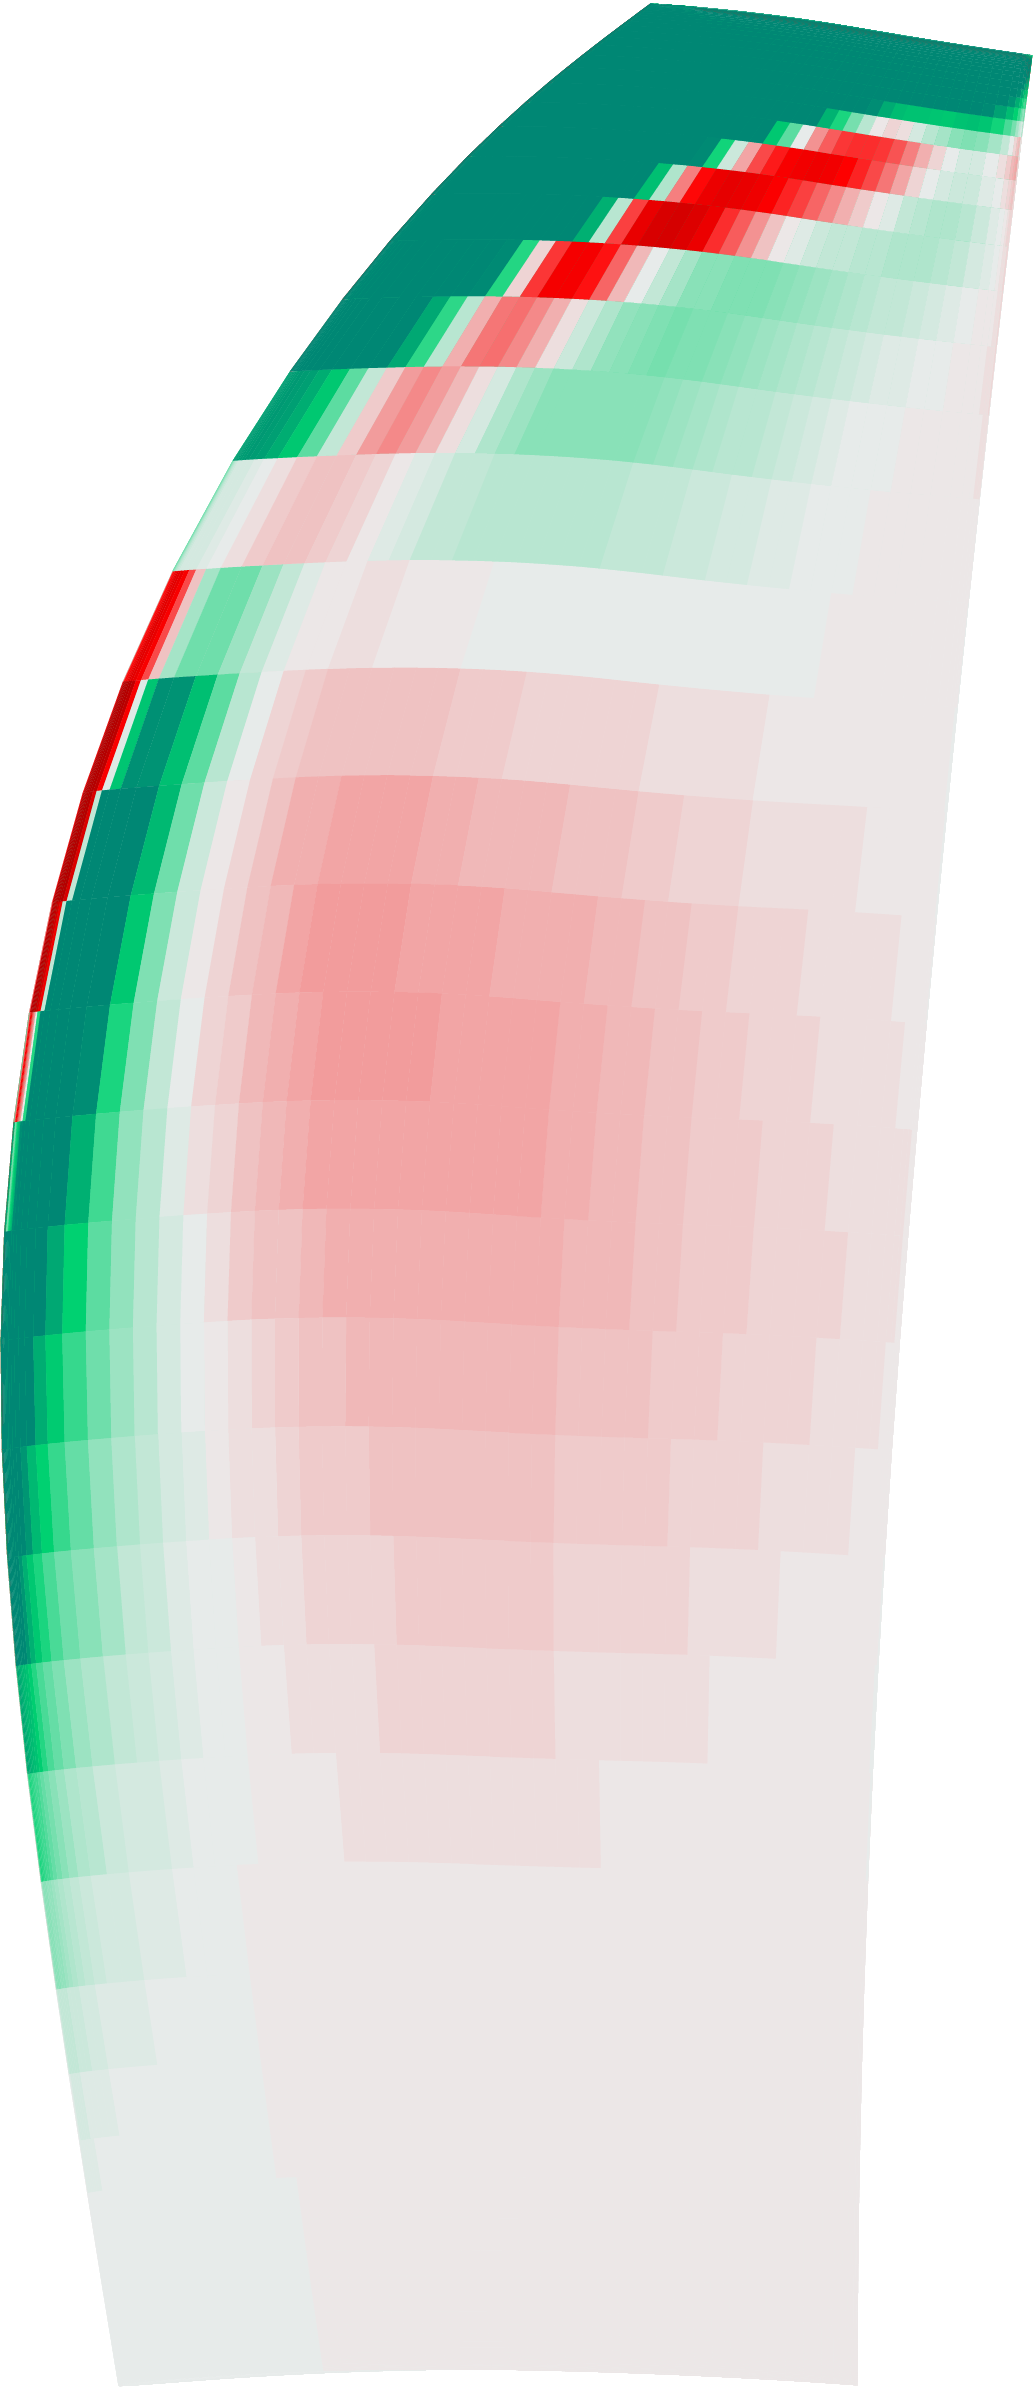
\includegraphics[width=0.12\textwidth]{DREAM_LS_HBT_N5_AEL_H1M2FD-1_roe3_sa_local_damping_SS.png}
   & 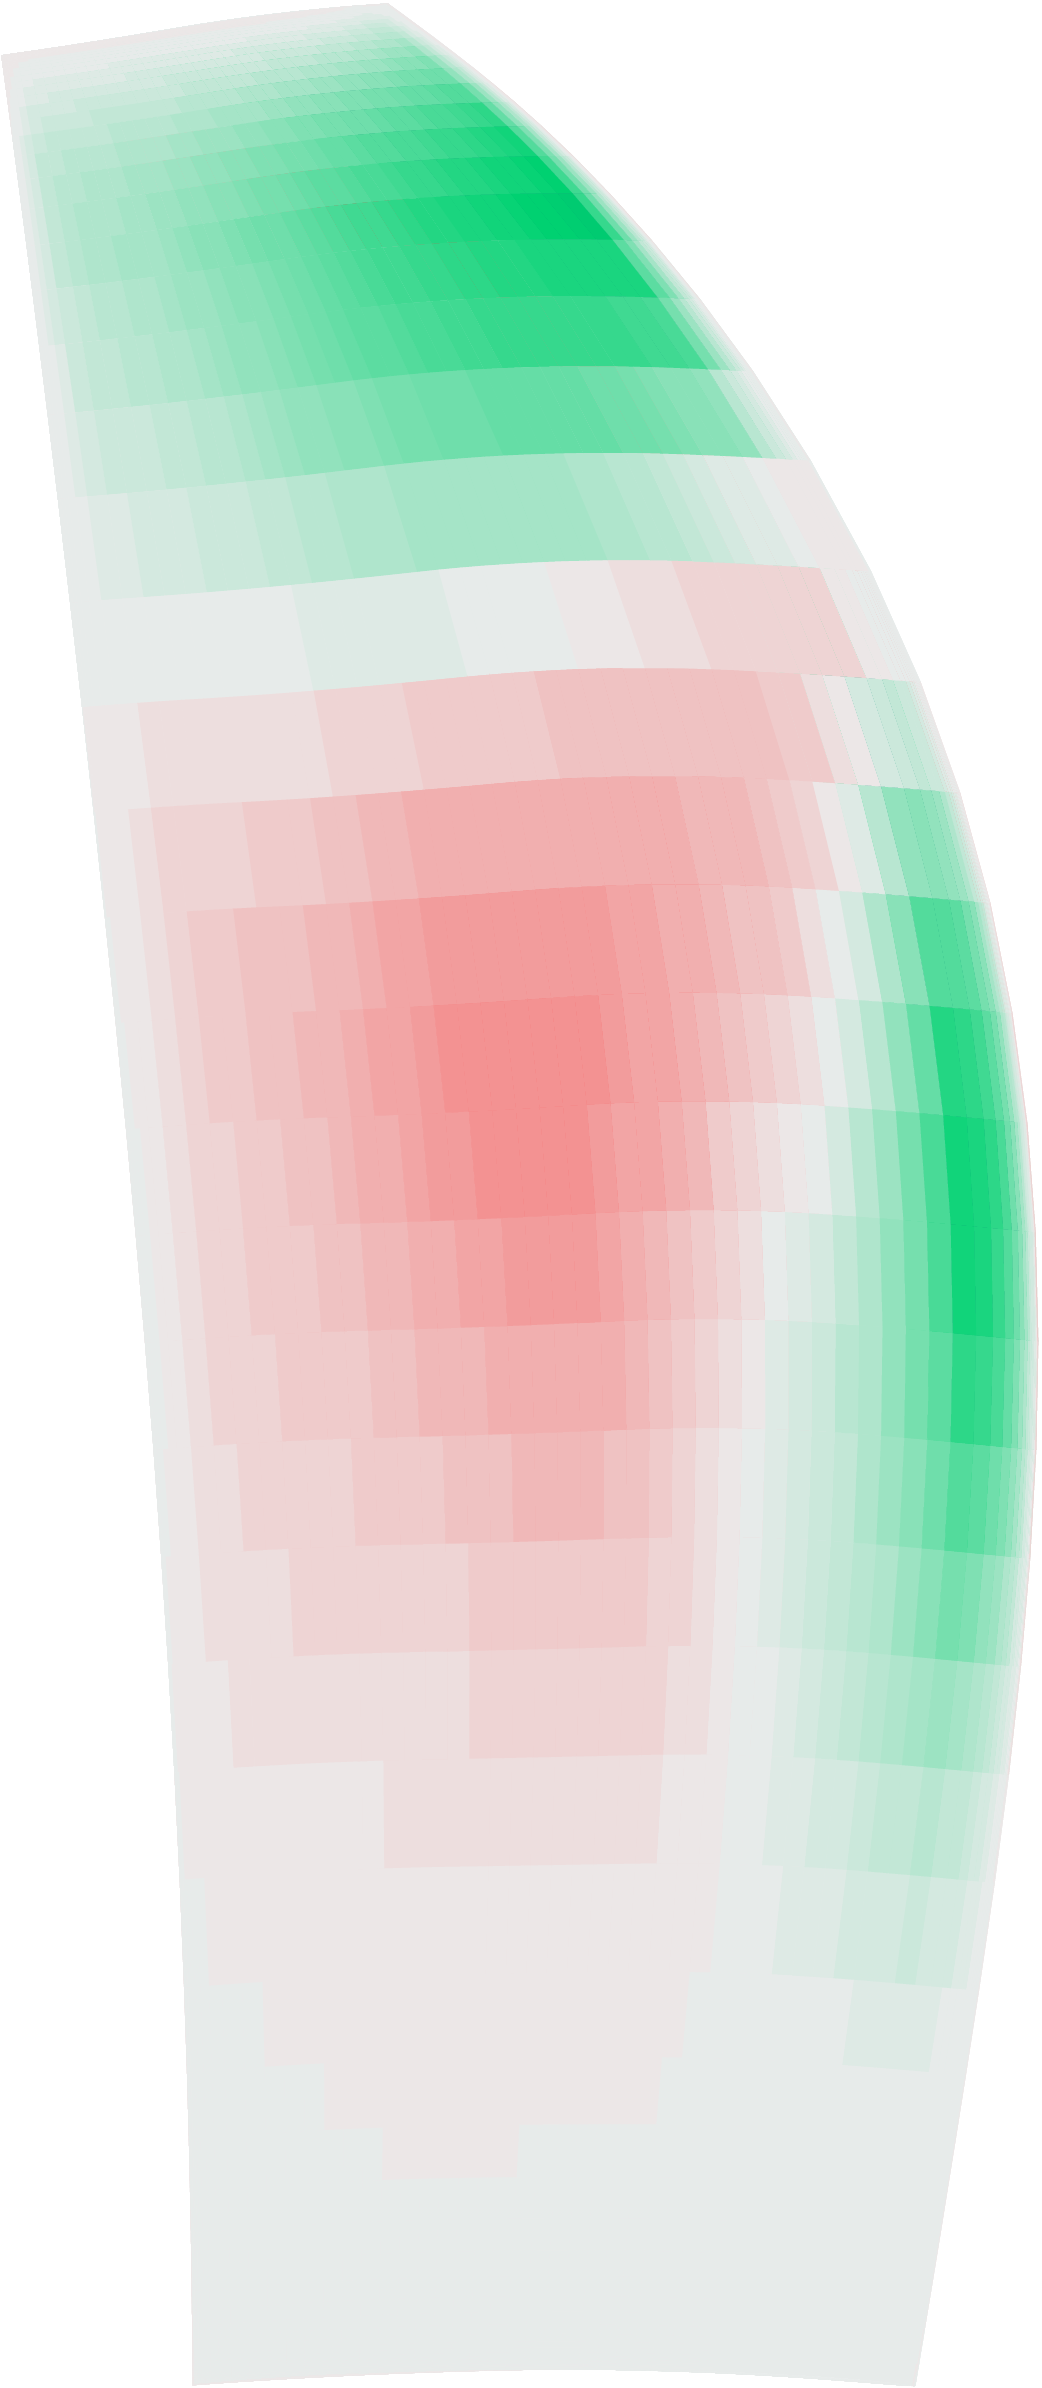
\includegraphics[width=0.12\textwidth]{DREAM_LS_HBT_N5_AEL_H1M2FD-1_roe3_sa_local_damping_PS.png}
   & 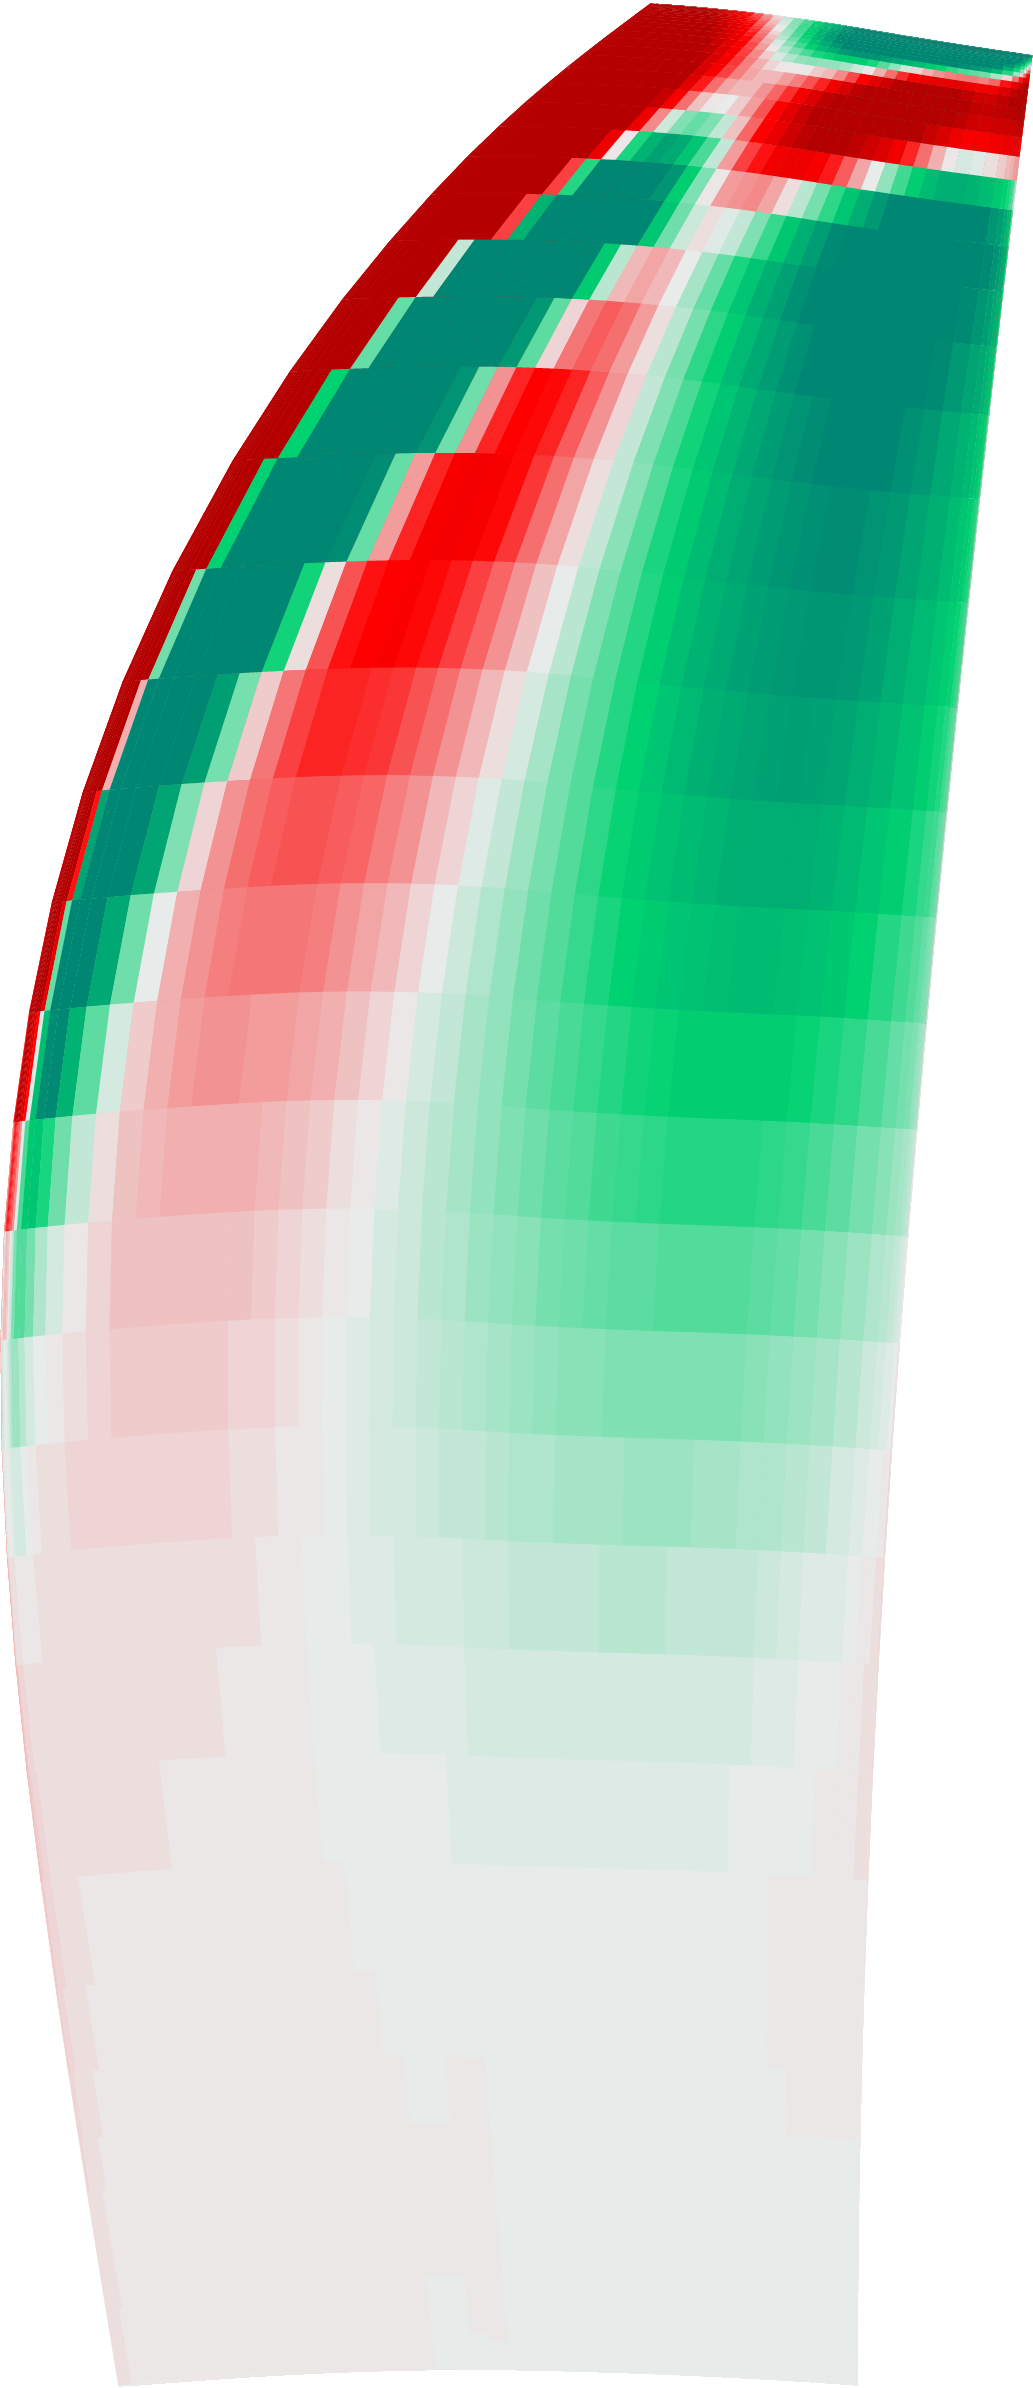
\includegraphics[width=0.12\textwidth]{DREAM_LS_HBT_N5_AEL_H1M1TD-1_roe3_sa_local_damping_SS.png}
   & 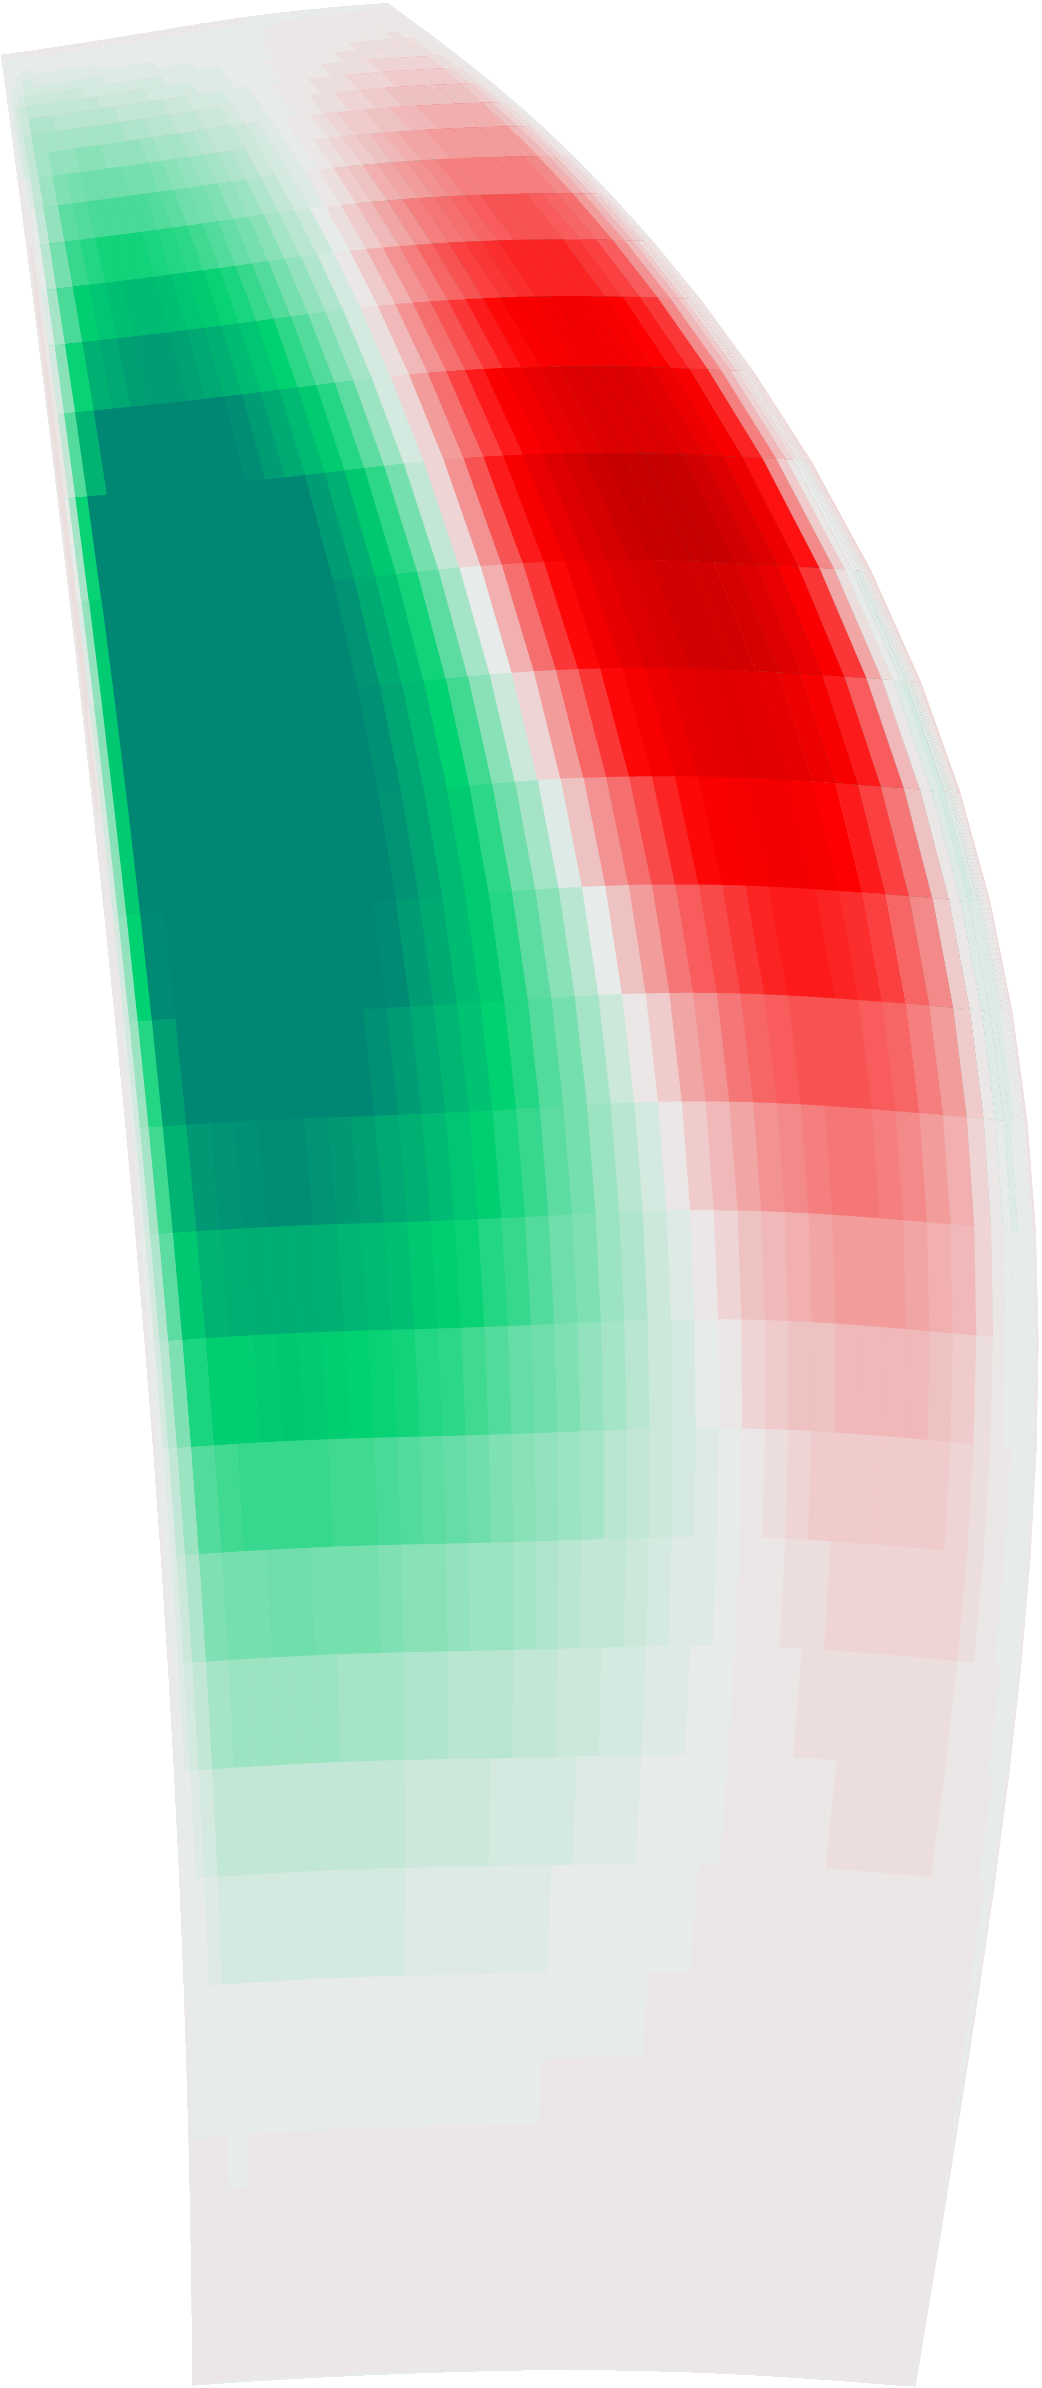
\includegraphics[width=0.12\textwidth]{DREAM_LS_HBT_N5_AEL_H1M1TD-1_roe3_sa_local_damping_PS.png} \\
   \rotatebox{90}{\quad\quad\quad IBPA $= 30^\circ$} 
   & 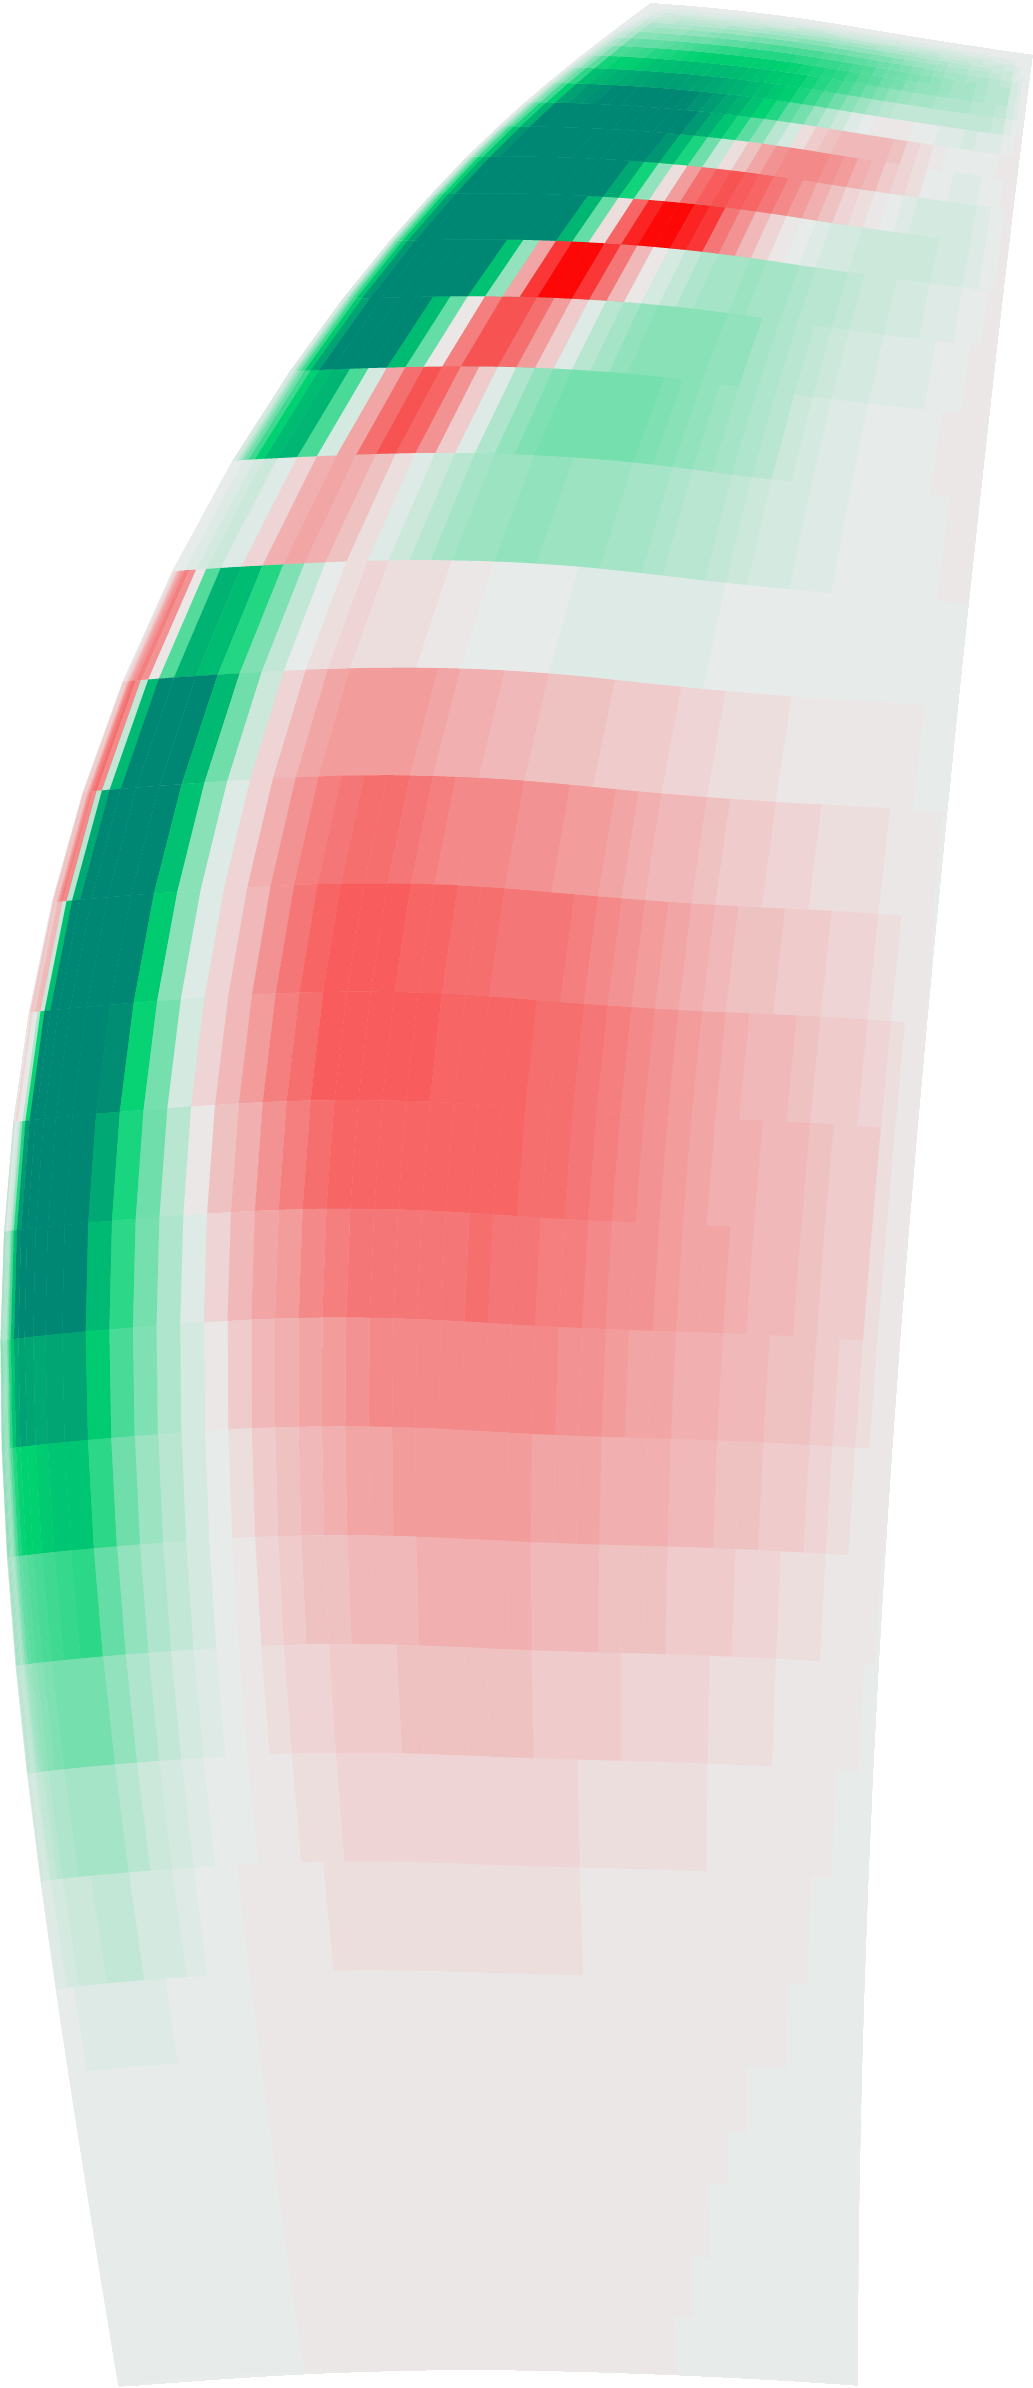
\includegraphics[width=0.12\textwidth]{DREAM_LS_HBT_N5_AEL_H1M2FD1_roe3_sa_local_damping_SS.png}
   & 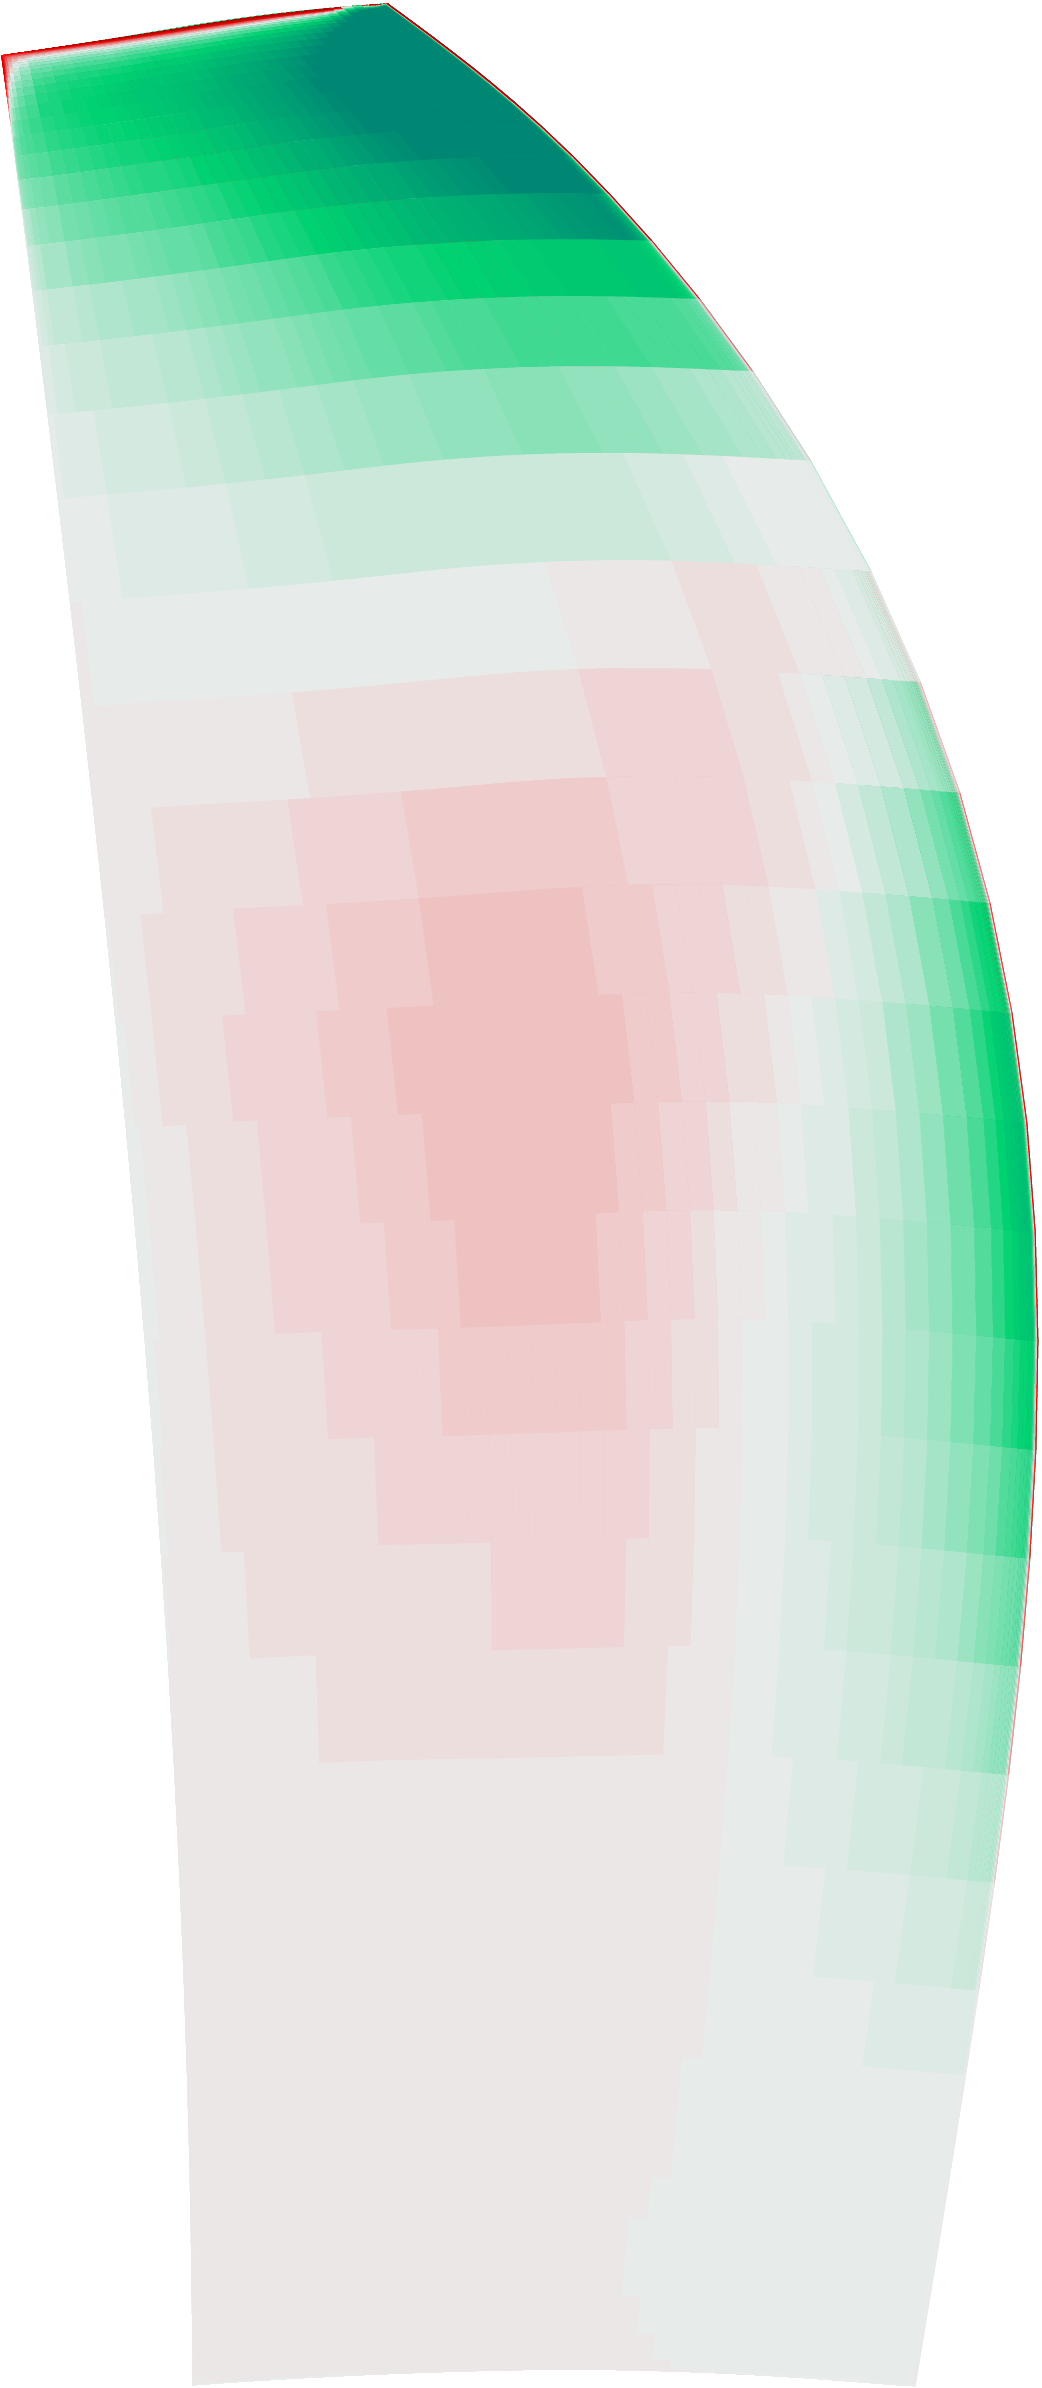
\includegraphics[width=0.12\textwidth]{DREAM_LS_HBT_N5_AEL_H1M2FD1_roe3_sa_local_damping_PS.png}
   & 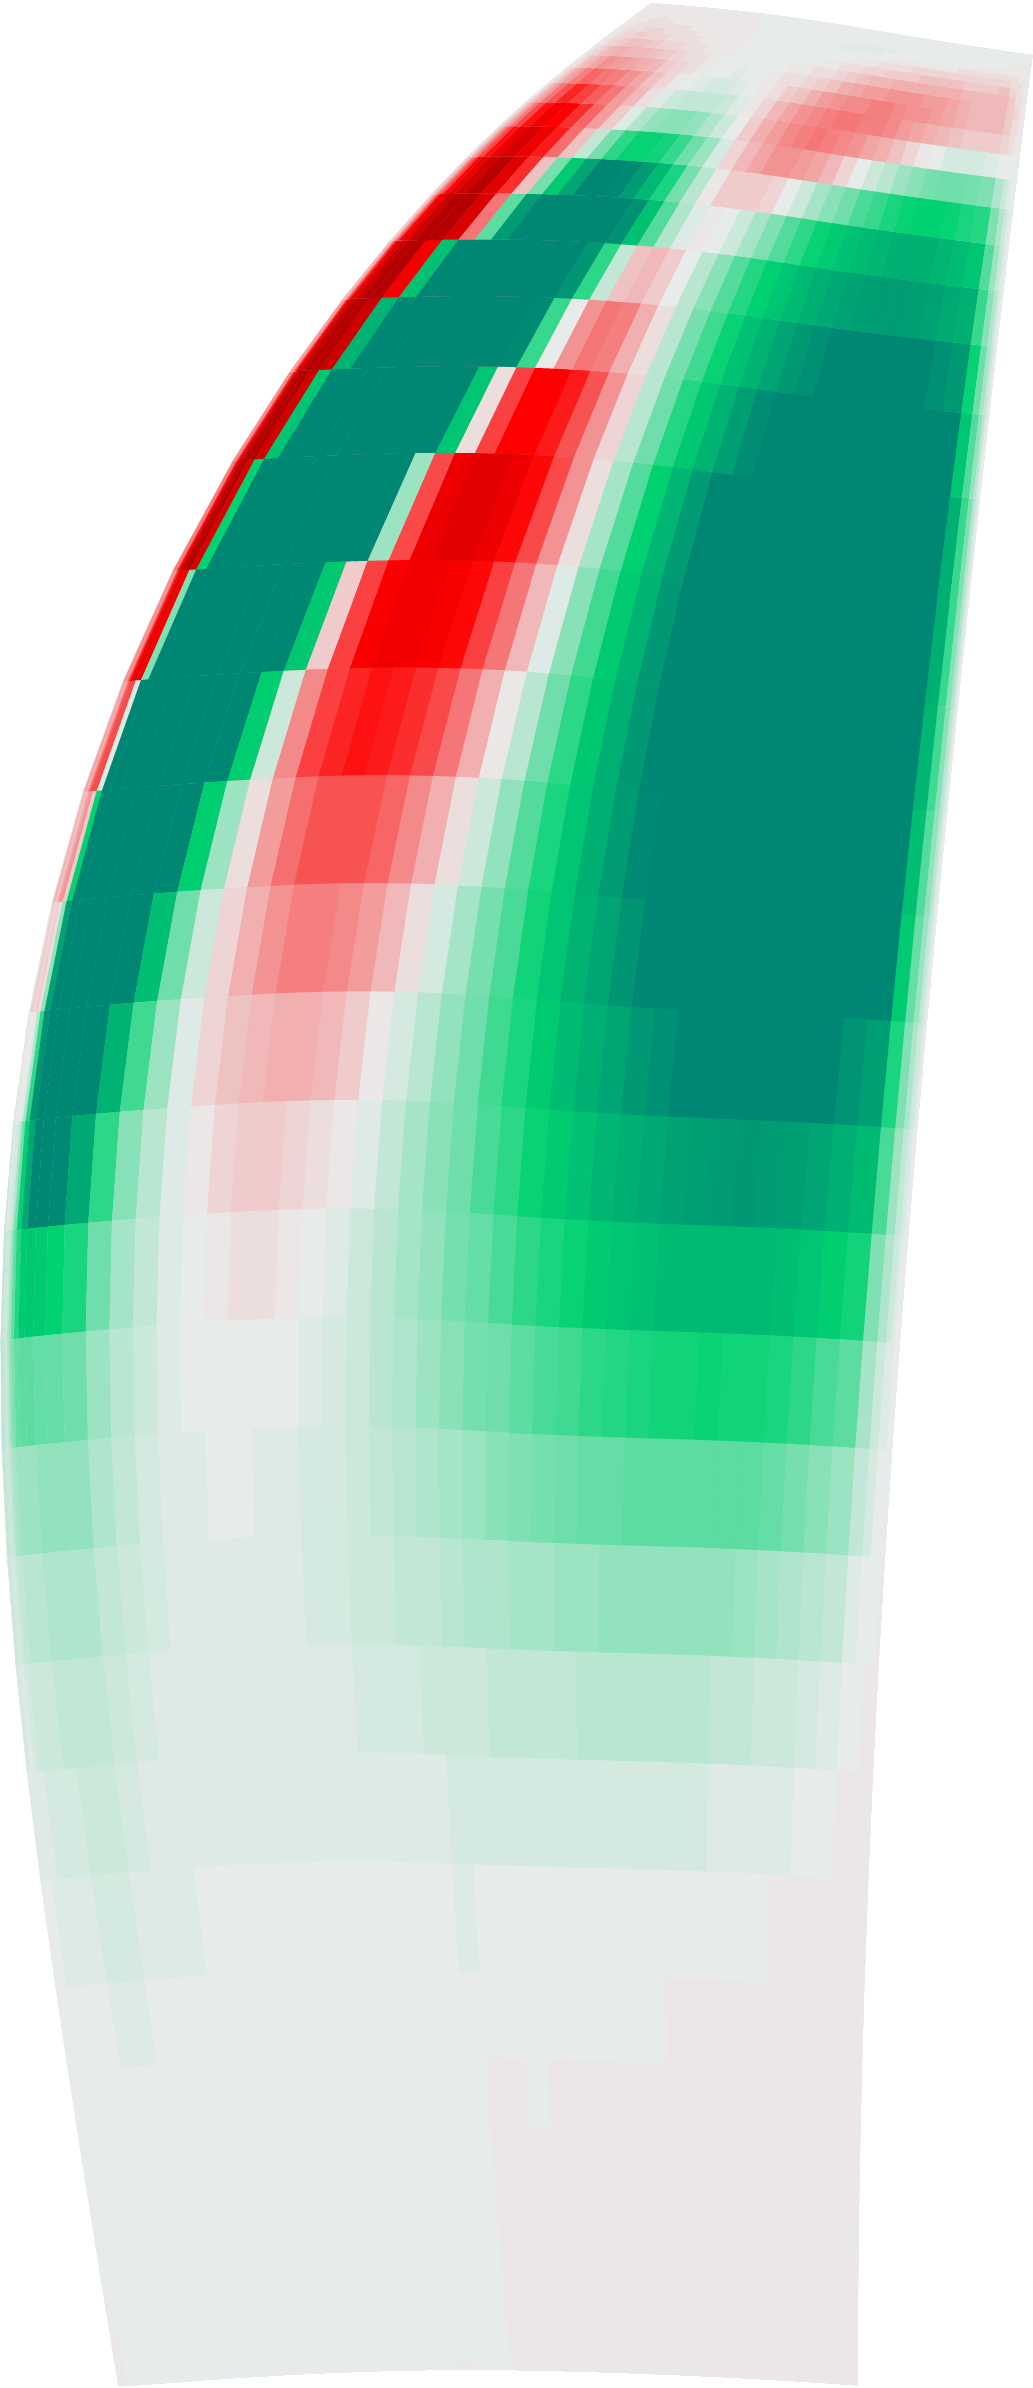
\includegraphics[width=0.12\textwidth]{DREAM_LS_HBT_N5_AEL_H1M1TD1_roe3_sa_local_damping_SS.png}
   & 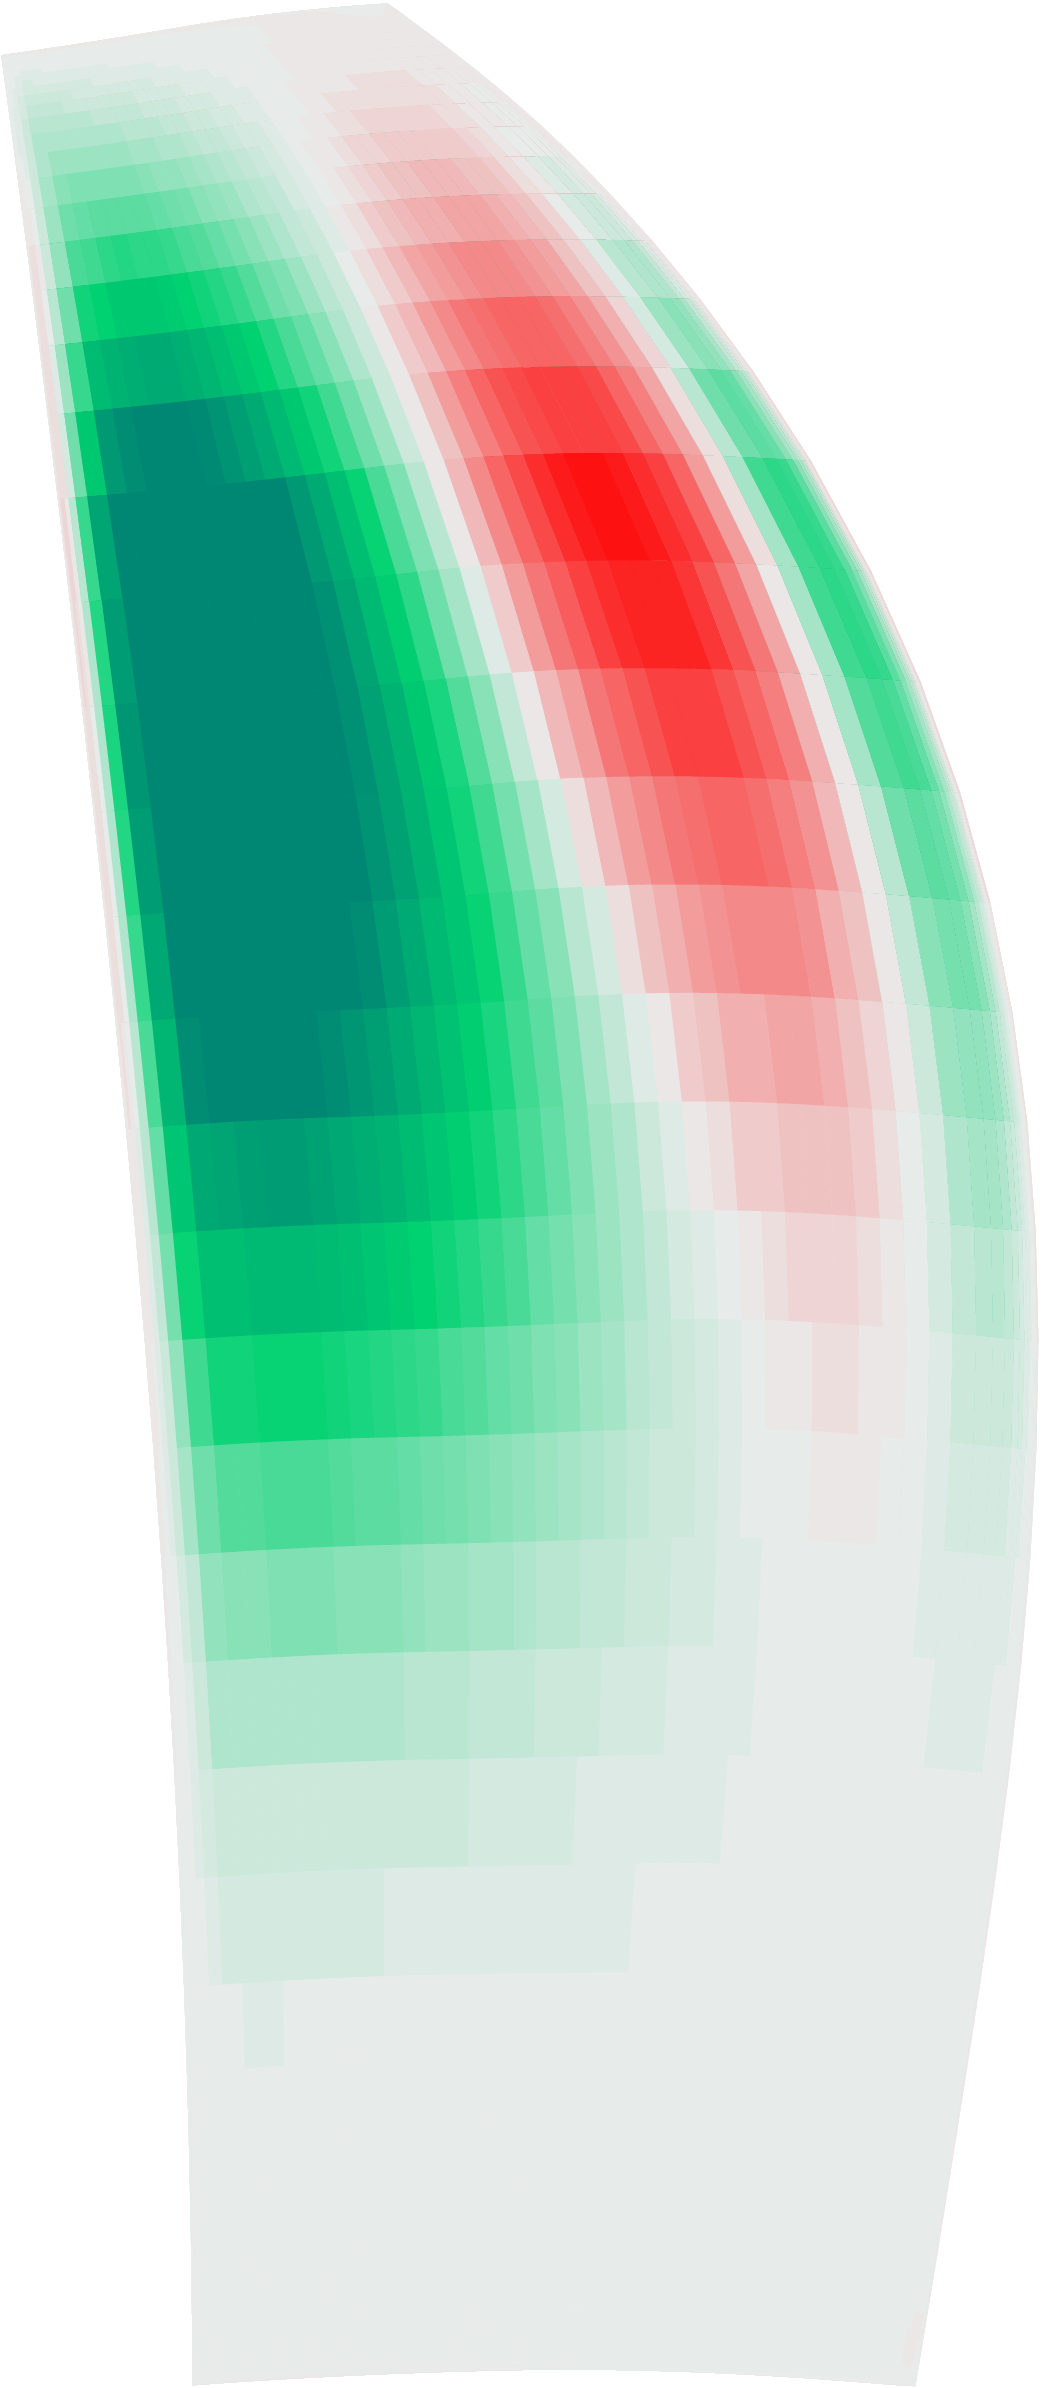
\includegraphics[width=0.12\textwidth]{DREAM_LS_HBT_N5_AEL_H1M1TD1_roe3_sa_local_damping_PS.png} \\
   \rotatebox{90}{\quad\quad\quad IBPA $= 60^\circ$} 
   & 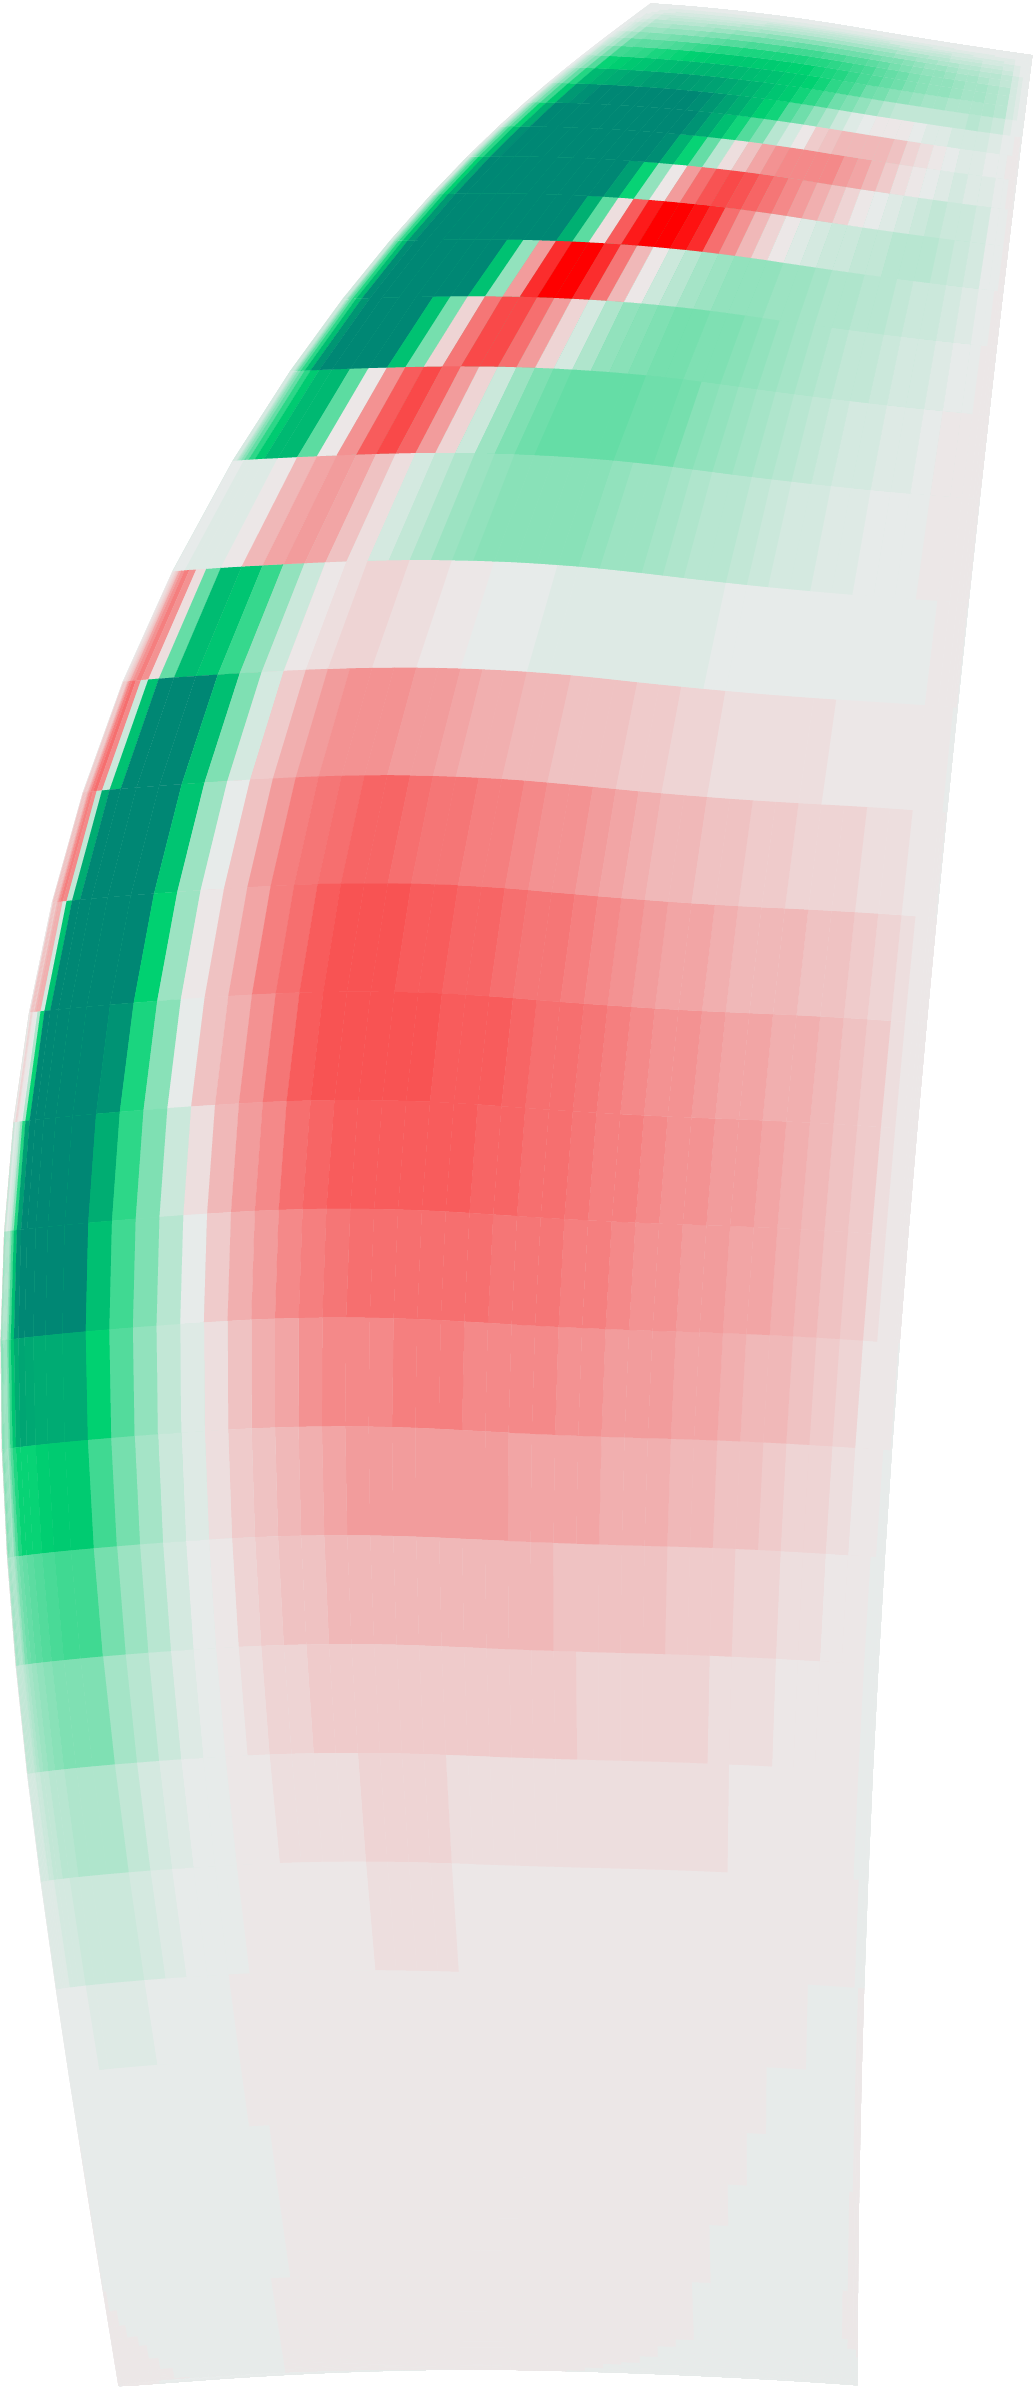
\includegraphics[width=0.12\textwidth]{DREAM_LS_HBT_N5_AEL_H1M2FD3_roe3_sa_local_damping_SS.png}
   & 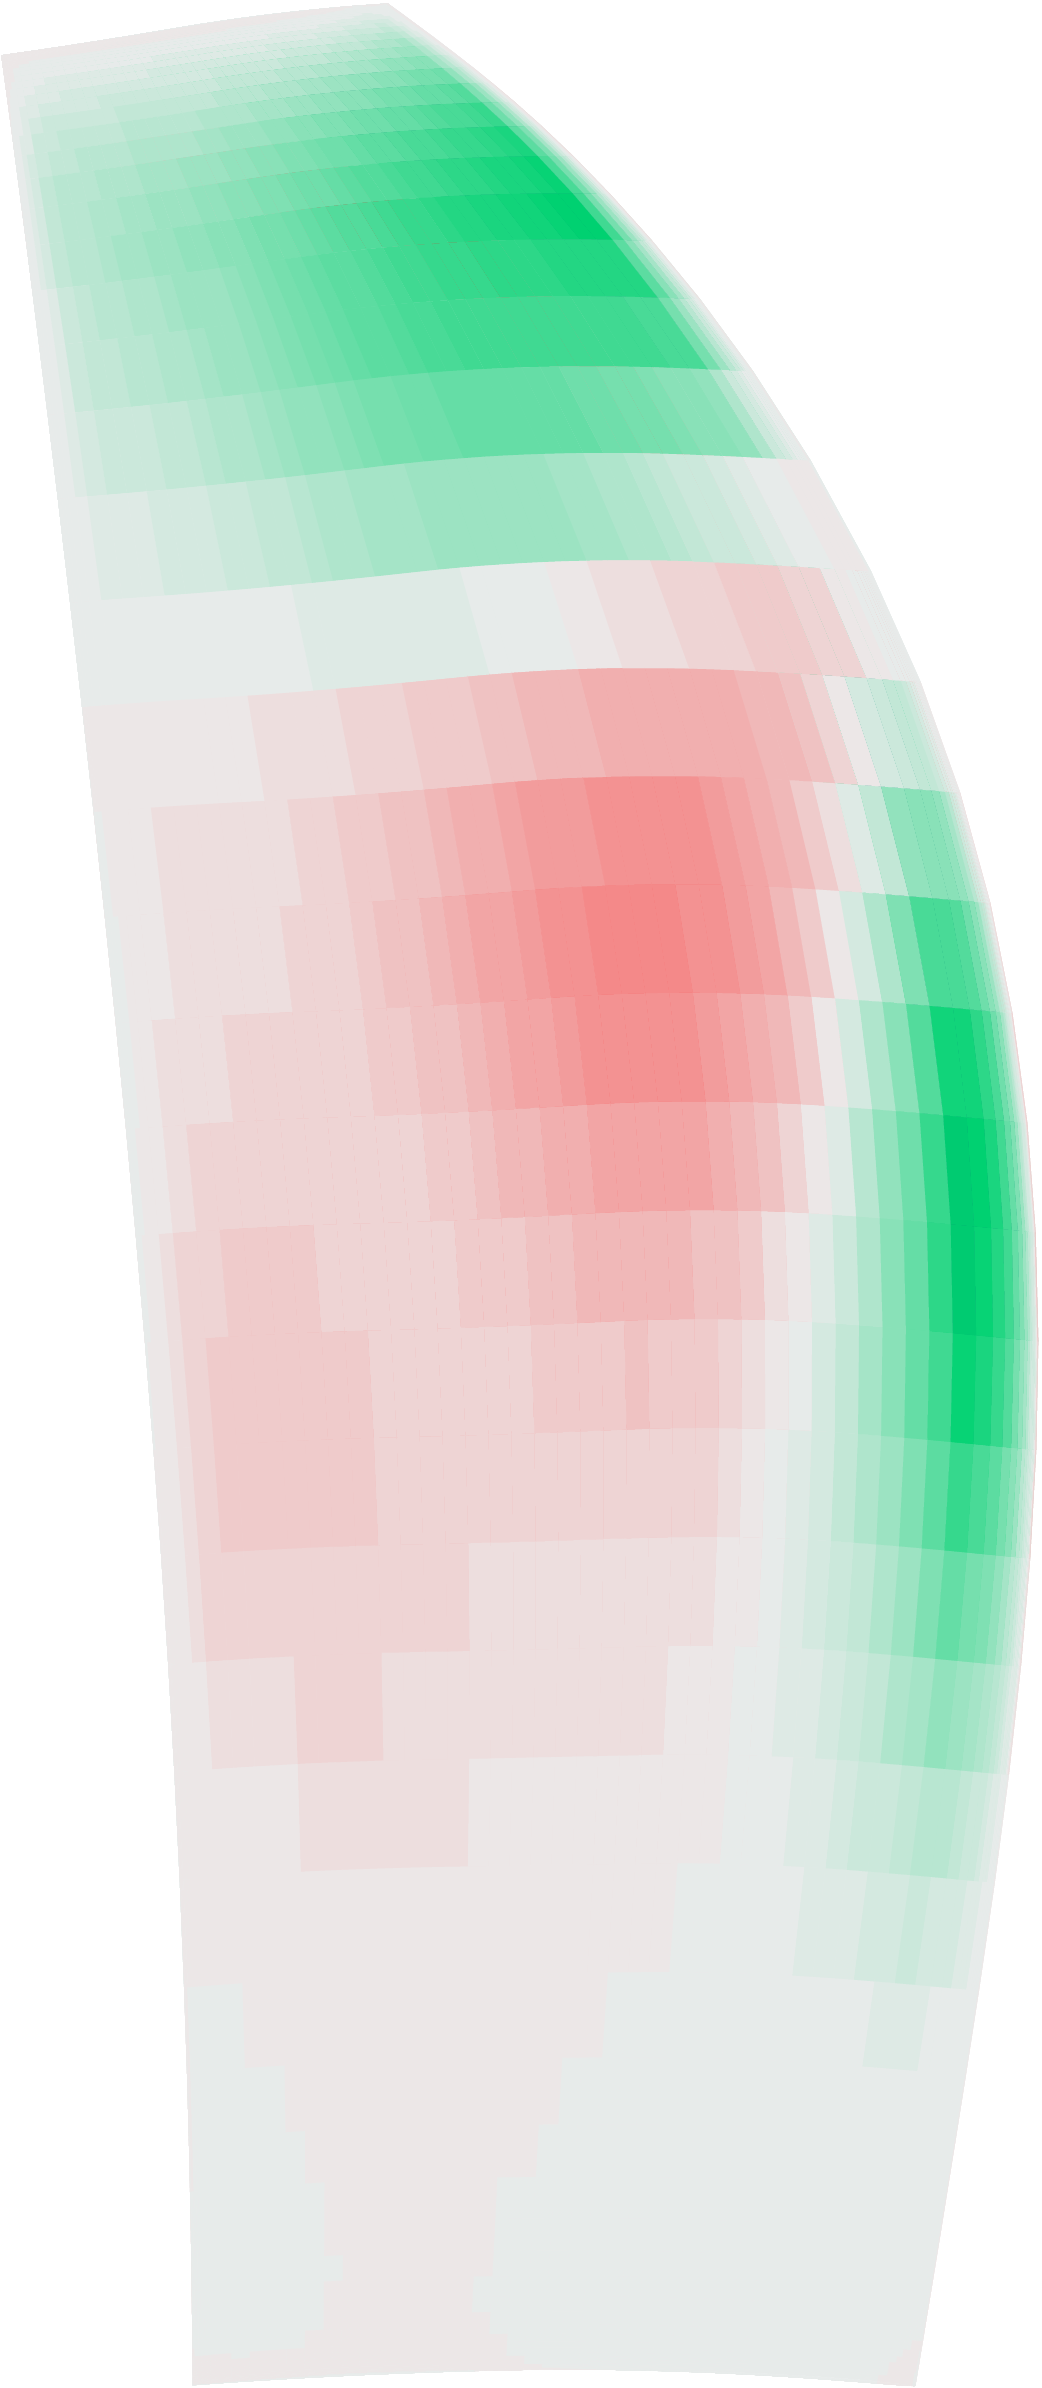
\includegraphics[width=0.12\textwidth]{DREAM_LS_HBT_N5_AEL_H1M2FD3_roe3_sa_local_damping_PS.png}
   & 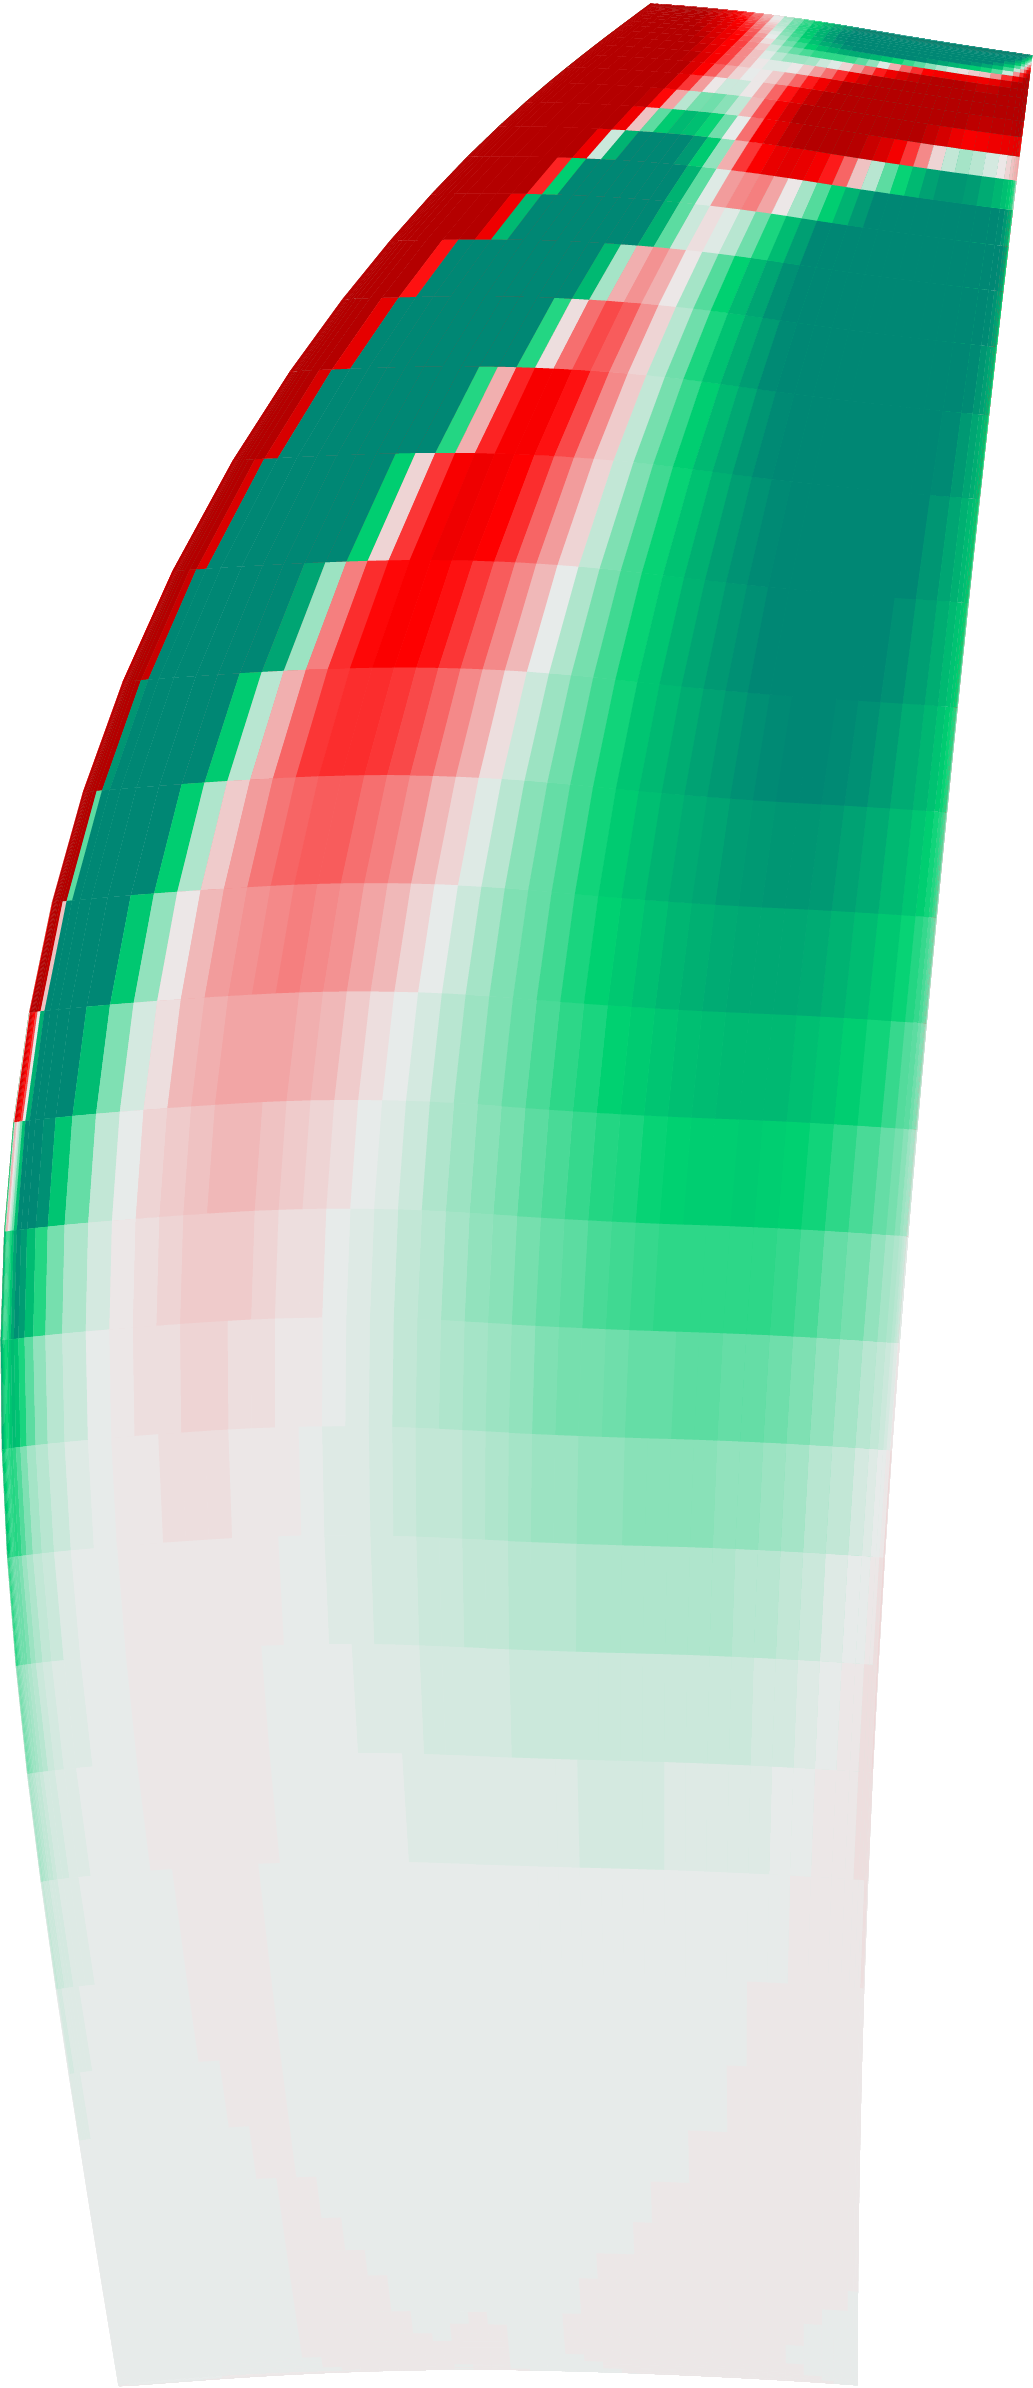
\includegraphics[width=0.12\textwidth]{DREAM_LS_HBT_N5_AEL_H1M1TD3_roe3_sa_local_damping_SS.png}
   & 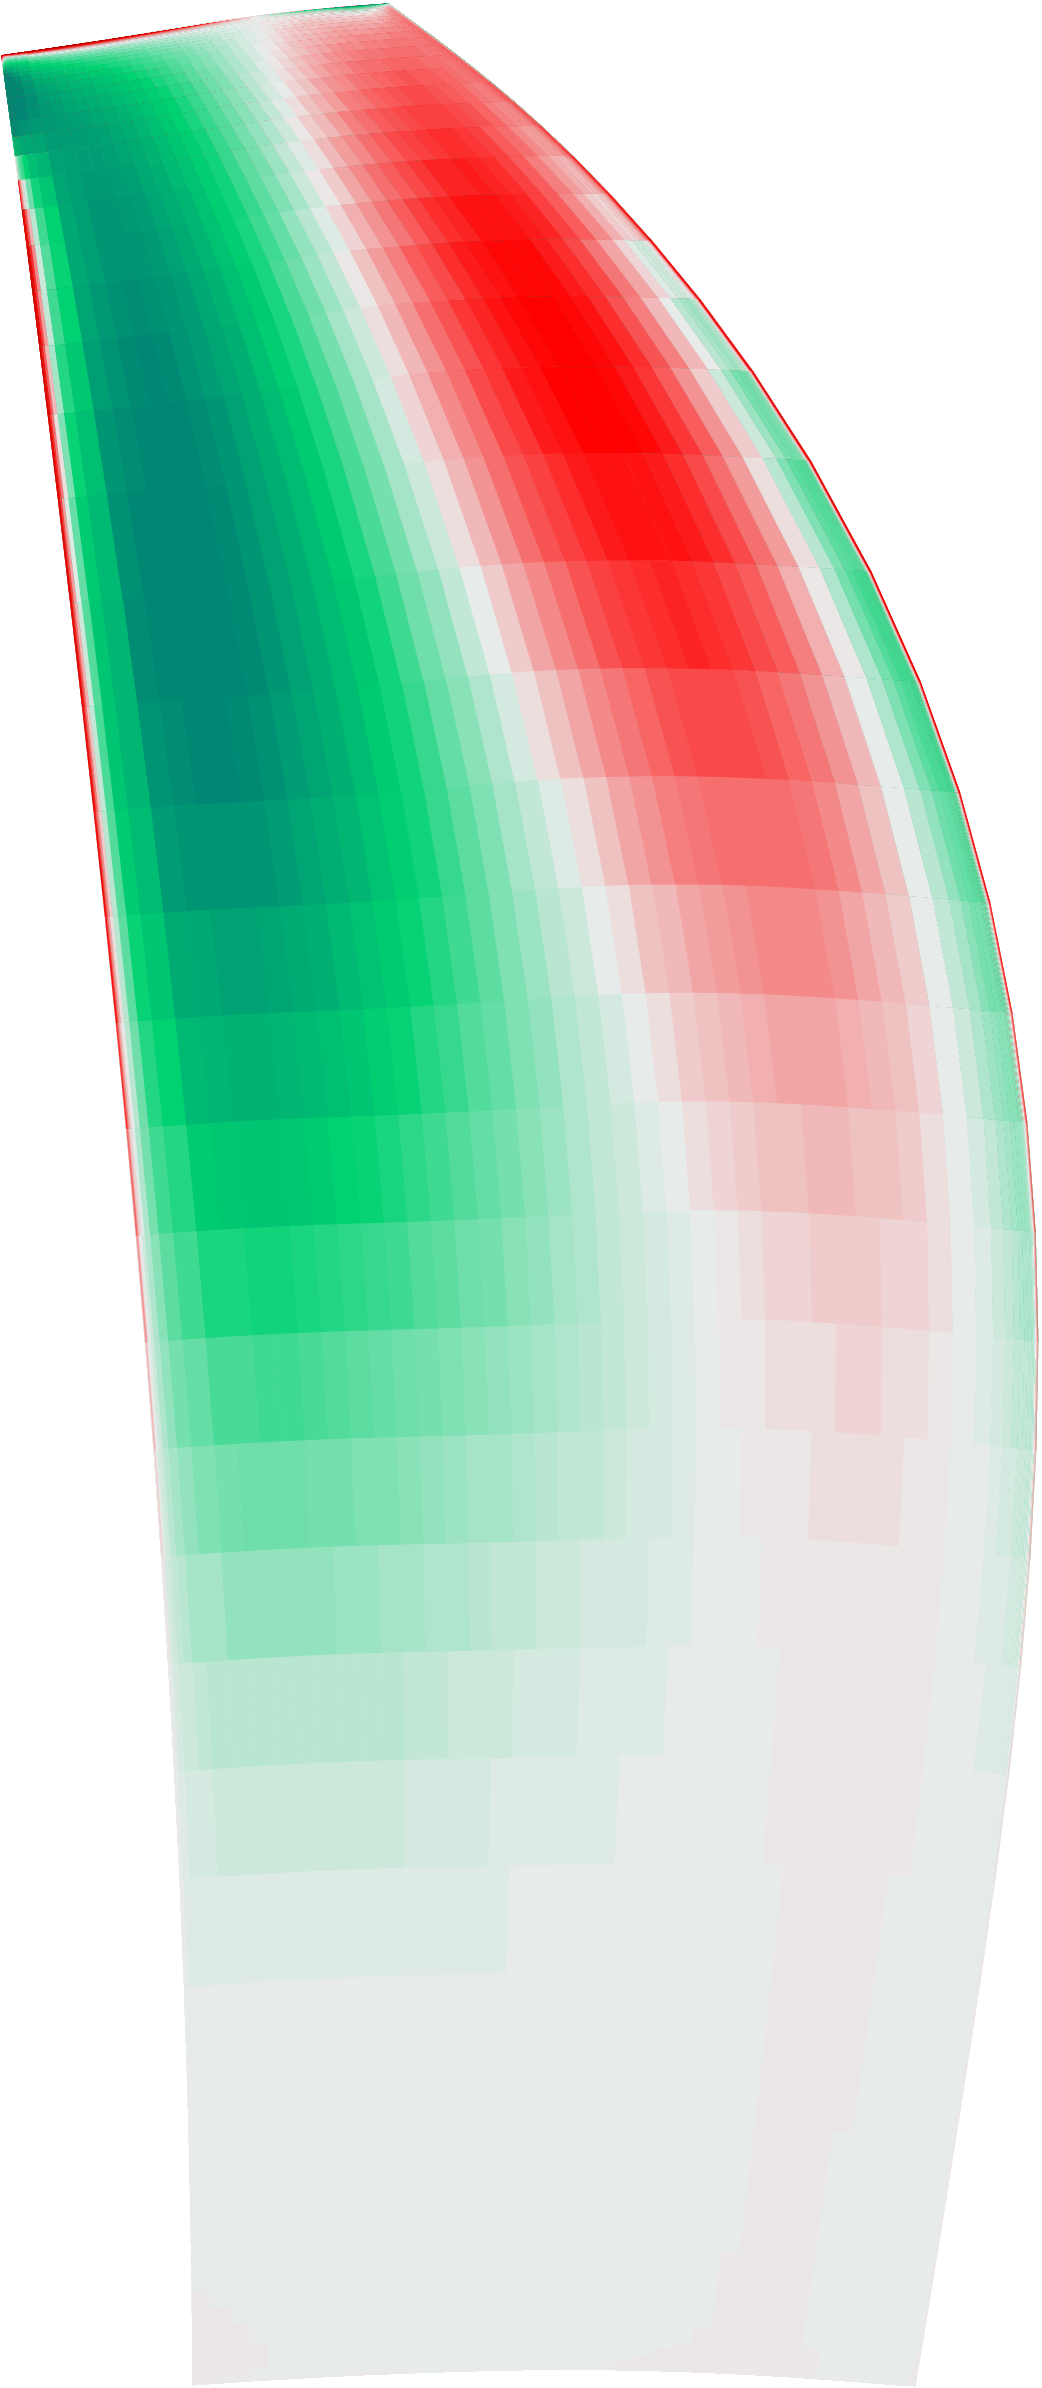
\includegraphics[width=0.12\textwidth]{DREAM_LS_HBT_N5_AEL_H1M1TD3_roe3_sa_local_damping_PS.png} \\
   & suction side & pressure side & suction side & pressure side \\
   \bottomrule
 \end{tabular}
 \caption{Low-speed isolated configuration: local damping for modes 2F and 1T.}
 \label{fig:dream_ls_ael_local_damping}
\end{figure}